\section*{Гармонический бустинг (Harmonic Boosting)}

Гармонический бустинг (Harmonic Boosting) представляет собой ансамблевый метод, целью которого является минимизация вклада моделей с высокой ошибкой путём взвешивания их предсказаний на основе гармонического среднего. Этот подход улучшает устойчивость ансамбля и снижает риск ухудшения качества из-за наличия "шумных" моделей.

\subsection*{Основная идея}

Гармоническое среднее даёт больший вес точным моделям и минимизирует влияние слабых или ошибочных предсказаний. Для \( n \) моделей ансамбля итоговое предсказание классификации вычисляется как:
\[
\hat{y} = \arg\max_{k} \left( \frac{n}{\sum_{i=1}^n \frac{1}{P_k(y_i)}} \right),
\]
где \( P_k(y_i) \) — вероятность принадлежности к классу \( k \), предсказанная \( i \)-й моделью.

Для регрессии итоговое предсказание:
\[
\hat{y} = \frac{n}{\sum_{i=1}^n \frac{1}{y_i}},
\]
где \( y_i \) — результат \( i \)-й модели.

\subsection*{Математическое обоснование}

Рассмотрим задачу регрессии. Пусть \( y_i \) — предсказание \( i \)-й модели, а \( e_i \) — её ошибка. Общая ошибка ансамбля определяется как:
\[
E = \frac{n}{\sum_{i=1}^n \frac{1}{e_i}}.
\]
Гармоническое среднее минимизирует \( E \), поскольку больший вес получают модели с меньшей ошибкой. Это свойство обеспечивает устойчивость ансамбля и снижает влияние "шумных" моделей.

Для классификации гармоническое среднее вероятностей используется в логарифмическом масштабе:
\[
\log P(C_k) = -\sum_{i=1}^n \frac{1}{\log P_k(y_i)}.
\]
Такой подход позволяет смягчить влияние моделей с крайне низкой вероятностью.

\subsection*{Алгоритм гармонического бустинга}

\textbf{Вход:}
\begin{itemize}
    \item Набор данных \( \mathcal{D} = \{(x_i, y_i)\}_{i=1}^m \),
    \item Количество слабых моделей \( T \),
    \item Функция потерь \( L(y, \hat{y}) \).
\end{itemize}

\textbf{Шаги алгоритма:}
\begin{enumerate}
    \item Инициализация ансамбля с первой моделью \( h_1 \), обученной на \( \mathcal{D} \).
    \item Вычисление весов для объектов в \( \mathcal{D} \) на основе обратной ошибки:
    \[
    w_j^{(t)} = \frac{1}{e_j^{(t)}},
    \]
    где \( e_j^{(t)} = L(y_j, h_t(x_j)) \).
    \item Построение новой модели \( h_{t+1} \) с учётом весов \( w_j^{(t)} \).
    \item Итоговое предсказание ансамбля:
    \[
    \hat{y} = \frac{n}{\sum_{i=1}^T \frac{1}{h_i(x)}}.
    \]
\end{enumerate}

\subsection*{Сравнение с другими методами бустинга}

В отличие от AdaBoost и градиентного бустинга, где обновление весов основывается на увеличении влияния сложных для классификации объектов, гармонический бустинг нацелен на минимизацию влияния моделей с высокой ошибкой. Это делает метод более устойчивым к выбросам и шуму.

\subsection*{Пример применения}

Рассмотрим задачу классификации на двух классах \( C_1 \) и \( C_2 \). Пусть ансамбль состоит из трёх моделей с вероятностями:
\[
P(C_1 | h_1) = 0.8, \quad P(C_1 | h_2) = 0.6, \quad P(C_1 | h_3) = 0.2.
\]
Итоговое предсказание для класса \( C_1 \) будет:
\[
P(C_1) = \frac{3}{\frac{1}{0.8} + \frac{1}{0.6} + \frac{1}{0.2}} \approx 0.44.
\]

\subsection*{Преимущества и ограничения}

\textbf{Преимущества:}
\begin{itemize}
    \item Устойчивость к шумным данным и выбросам.
    \item Минимизация вклада моделей с высокой ошибкой.
\end{itemize}

\textbf{Ограничения:}
\begin{itemize}
    \item Высокая вычислительная сложность.
    \item Чувствительность к выбору базовых моделей.
\end{itemize}

\section*{Задачи}

\subsection*{Задача 1: Теоретическое доказательство свойства гармонического среднего}

Докажите, что гармоническое среднее минимизирует влияние на общую ошибку моделей с большими значениями ошибки \( e_i \).

\textbf{Решение:}
\begin{enumerate}
    \item Запишем общую ошибку ансамбля:
    \[
    E = \frac{n}{\sum_{i=1}^n \frac{1}{e_i}}.
    \]
    \item Рассмотрим случай, когда одна из ошибок \( e_i \) существенно больше других. Тогда:
    \[
    \sum_{i=1}^n \frac{1}{e_i} \approx \frac{1}{e_1} + \frac{1}{e_2} + \ldots + \frac{1}{e_k} + \frac{1}{e_{\text{max}}},
    \]
    где \( e_{\text{max}} \gg e_k \).
    \item Гармоническое среднее делает вклад \( \frac{1}{e_{\text{max}}} \) минимальным, сохраняя значительное влияние \( \frac{1}{e_k} \), что уменьшает общий эффект высоких ошибок на ансамбль.
\end{enumerate}

\subsection*{Задача 2: Алгоритм на данных}

Даны предсказания трёх моделей на выборке:
\[
P(C_1 | h_1) = [0.9, 0.3, 0.6], \quad P(C_1 | h_2) = [0.8, 0.4, 0.7], \quad P(C_1 | h_3) = [0.7, 0.2, 0.5].
\]
Используя гармонический бустинг, вычислите итоговое предсказание ансамбля.

\textbf{Решение:}
\begin{enumerate}
    \item Рассчитаем гармоническое среднее для каждого объекта:
    \[
    P(C_1 | x_1) = \frac{3}{\frac{1}{0.9} + \frac{1}{0.8} + \frac{1}{0.7}} \approx 0.8,
    \]
    \[
    P(C_1 | x_2) = \frac{3}{\frac{1}{0.3} + \frac{1}{0.4} + \frac{1}{0.2}} \approx 0.26,
    \]
    \[
    P(C_1 | x_3) = \frac{3}{\frac{1}{0.6} + \frac{1}{0.7} + \frac{1}{0.5}} \approx 0.57.
    \]
    \item Итоговое предсказание: \( [0.8, 0.26, 0.57] \).
\end{enumerate}

\subsection*{Задача 3: Сравнение с арифметическим средним}

Сравните результаты гармонического и арифметического средних для трёх моделей с предсказаниями:
\[
P(C_1 | h_1) = 0.9, \quad P(C_1 | h_2) = 0.1, \quad P(C_1 | h_3) = 0.8.
\]

\textbf{Решение:}
\begin{enumerate}
    \item \textbf{Арифметическое среднее:}
    \[
    P(C_1) = \frac{0.9 + 0.1 + 0.8}{3} = 0.6.
    \]
    \item \textbf{Гармоническое среднее:}
    \[
    P(C_1) = \frac{3}{\frac{1}{0.9} + \frac{1}{0.1} + \frac{1}{0.8}} \approx 0.27.
    \]
    \item Гармоническое среднее уменьшает вклад модели \( h_2 \) с высокой ошибкой \( (P(C_1) = 0.1) \), что приводит к более устойчивому предсказанию.
\end{enumerate}

\section{Градиентный бустинг}

\subsection{Что такое градиентный бустинг и его история}

Градиентный бустинг — это метод машинного обучения, основанный на идее последовательного обучения ансамбля слабых моделей (чаще всего деревьев решений) с использованием градиентного спуска для минимизации заданной функции потерь. Основная цель этого метода — построить сильную модель, которая последовательно улучшает свои предсказания, исправляя ошибки предыдущих шагов.

Идея градиентного бустинга была предложена Джереми Фридманом в 1999 году в его работе "Greedy Function Approximation: A Gradient Boosting Machine". Этот метод стал обобщением алгоритма AdaBoost, который также строит ансамбль из слабых моделей, но оптимизирует экспоненциальную функцию потерь. Градиентный бустинг же позволил использовать произвольные дифференцируемые функции потерь, такие как квадратичная ошибка для регрессии или логистическая функция для классификации. Эта гибкость сделала градиентный бустинг одним из самых мощных методов для решения задач прогнозирования.

\subsection{Объяснение с лекции К.В.Воронцова}

Рассмотрим уже пройденный линейный ансамбль базовых алгоритмов $b_t$ из семейства $\mathcal{B}$:
\[
a_T(x) = \sum_{t=1}^{T} \alpha_t b_t(x), \quad x \in \textbf{X}, \; b_t : \textbf{X} \to \mathbb{R}, \; \alpha_t \in \mathbb{R}^+.
\]

Эвристика: обучаем $\alpha_T$, $b_T$ при фиксированных предыдущих.

Критерий качества с заданной \textbf{гладкой} функцией потерь $L(b, y)$:

\[
Q(\alpha, b; X^\ell) = \sum_{i=1}^\ell L\left(\sum_{t=1}^{T-1} \alpha_t b_t(x_i) + \alpha b(x_i), y_i \right) \to \min_{\alpha, b}.
\]

Цель построить следующий алгоритм $b(x_i)$ и подобрать к нему $\alpha$, на основе предыдущих t алгоритмов $\alpha_t b_t(x_i)$.  
Будем называть $\alpha_t b_t(x_i)$ - текущее приближение, и $\alpha b(x_i)$ - следующее приближение. 

Можем рассматривать это как минимизацию в другом пространстве: $Q(f) \to \min$, $f \in \mathbb{R}^\ell$. Предположим, что в этом пространстве мы можем производить градиентный спуск, тогда выбор приближения будет выглядеть так:

\begin{align*}
a_{0,i} & := \text{начальное приближение}, \\
a_{T,i} & := a_{T-1,i} - \alpha g_i, \quad i = 1, \dots, \ell, \\
g_i & = L'_f(a_{T-1,i}, y_i) \quad \text{(компоненты вектора градиента)}, \\
\alpha & \text{--- градиентный шаг}.
\end{align*}

Это эквивалентно добавлению одного базового алгоритма:
\[
a_{T,i} := a_{T-1,i} + \alpha b(x_i), \quad i = 1, \dots, \ell.
\]

\textbf{Идея:} найти такой базовый алгоритм $b_T \in \mathcal{B}$, чтобы вектор $(b_T(x_i))_{i=1}^\ell$ аппроксимировал вектор антиградиента $(-g_i)_{i=1}^\ell$:
\[
b_T := \arg\min_{b \in \mathcal{B}} \sum_{i=1}^\ell \left(b(x_i) + g_i \right)^2.
\]

\textbf{Алгоритм градиентного бустинга}

Вход: обучающая выборка $X^\ell$; параметр $T$.

Выход: базовые алгоритмы и их веса $\alpha_t b_t$, $t = 1, \dots, T$.

\textbf{Инициализация:}
\[
a_{0,i} := 0, \quad i = 1, \dots, \ell.
\]

\textbf{Для всех} $t = 1, \dots, T$:
\begin{enumerate}
    \item Базовый алгоритм, приближающий антиградиент:
    \[
    b_t := \arg\min_{b \in \mathcal{B}} \sum_{i=1}^\ell \left(b(x_i) + L'(a_{t-1,i}, y_i) \right)^2.
    \]
    \item Задача одномерной минимизации:
    \[
    \alpha_t := \arg\min_{\alpha > 0} \sum_{i=1}^\ell L(a_{t-1,i} + \alpha b_t(x_i), y_i).
    \]
    \item Обновление вектора значений на объектах выборки:
    \[
    a_{t,i} := a_{t-1,i} + \alpha_t b_t(x_i), \quad i = 1, \dots, \ell.
    \]
\end{enumerate}

Каждый следующий базовый алгоритм обучается так, чтобы по возможности исправить ошибки предыдущих алгоритмов.

\subsection{Классическая аналогия с гольфом}

Представьте себе игру в гольф: игрок должен довести мяч до лунки. Первый удар обычно самый сильный и приблизительно доставляет мяч в район цели. Однако этого недостаточно, чтобы загнать мяч в лунку. Следующие удары — более точные и тонкие — корректируют траекторию, пока мяч не окажется в нужной точке.

Градиентный бустинг работает по аналогичному принципу. Изначально модель делает "грубое" предсказание (аналог первого удара в гольфе). Затем на каждом последующем шаге слабые модели "подталкивают" результат в сторону оптимума, исправляя ошибки предыдущих шагов. Эти корректировки можно рассматривать как попытки уменьшить расстояние между текущим предсказанием и истинным ответом (целевой меткой). Эта аналогия помогает интуитивно понять, как небольшие шаги градиентного спуска приближают модель к минимизации функции потерь.

\subsection{Применимость градиентного бустинга}

Градиентный бустинг применяется в широком спектре задач машинного обучения благодаря своей гибкости и высокой эффективности. Среди основных областей применения можно выделить:

\begin{itemize}
    \item \textbf{Классификация:} задачи, где нужно распределить объекты по классам, например, выявление мошеннических транзакций, прогнозирование оттока клиентов или медицинская диагностика.
    \item \textbf{Регрессия:} задачи, где нужно предсказать численное значение, такие как прогнозирование спроса, цены на рынке или уровня загрязнения воздуха.
    \item \textbf{Ранжирование:} задачи, где важно упорядочить объекты по степени их важности, например, поисковые системы или рекомендательные системы.
    \item \textbf{Обработка категориальных данных:} современные реализации, такие как CatBoost, значительно упростили работу с категориальными признаками, что делает градиентный бустинг полезным для анализа данных с такими особенностями.
\end{itemize}

Благодаря своей способности работать с разнородными признаками, поддержке пользовательских функций потерь и встроенным механизмам борьбы с переобучением, градиентный бустинг стал основным инструментом для построения производительных моделей в индустрии.

\subsection{Задачи для практики}

\subsubsection{Задача 1: Оптимизация базового алгоритма}

На шаге $t$ градиентного бустинга известны антиградиенты $-g_i$ для объектов $x_i$. Пусть $g_i = \hat{y}_{t-1}(x_i) - y_i$.  
Требуется построить базовый алгоритм $b_t(x)$, который минимизирует выражение:
\[
\sum_{i=1}^\ell (b_t(x_i) + g_i)^2.
\]
Найдите оптимальное значение $b_t(x_i)$ для каждого объекта $x_i$.

\textbf{Решение:}

Развернем выражение:
\[
\sum_{i=1}^\ell (b_t(x_i) + g_i)^2 = \sum_{i=1}^\ell b_t^2(x_i) + 2b_t(x_i)g_i + g_i^2.
\]
Оптимизируем по $b_t(x_i)$, приравняв производную к нулю:
\[
\frac{\partial}{\partial b_t(x_i)} \left(b_t^2(x_i) + 2b_t(x_i)g_i \right) = 2b_t(x_i) + 2g_i = 0.
\]
Отсюда:
\[
b_t(x_i) = -g_i.
\]

\textbf{Ответ:} $b_t(x_i) = -g_i$.

\subsubsection{Задача 2: Влияние параметра $\alpha$}

В градиентном бустинге используется коэффициент $\alpha_t$, определяющий, насколько сильно предсказания обновляются на каждом шаге:
\[
\hat{y}_t(x_i) = \hat{y}_{t-1}(x_i) + \alpha_t b_t(x_i).
\]
Объясните, как $\alpha_t$ влияет на процесс обучения и какие последствия имеет слишком маленькое или слишком большое значение $\alpha_t$.

\textbf{Решение:}

Параметр $\alpha_t$ регулирует величину обновлений предсказаний:
\begin{itemize}
    \item Если $\alpha_t$ слишком \textbf{маленькое}, обновления будут незначительными. Это может привести к медленной сходимости модели, так как процесс обучения станет более долгим.
    \item Если $\alpha_t$ слишком \textbf{большое}, модель будет стремиться к переобучению. Это связано с тем, что большие обновления могут чрезмерно акцентировать внимание на текущих ошибках, ухудшая обобщающую способность модели.
\end{itemize}

На практике $\alpha_t$ подбирается либо эмпирически, либо используется небольшой фиксированный шаг (например, 0.1), чтобы контролировать обучение и избежать резких изменений.

\textbf{Ответ:} $\alpha_t$ определяет баланс между скоростью обучения и устойчивостью модели. Малые значения $\alpha_t$ обеспечивают стабильность, большие — ускоряют обучение, но могут привести к переобучению.

\subsubsection{Задача 3: Отрицательные значения на тесте}

Может ли модель градиентного бустинга, обученная на выборке с исключительно положительными значениями признаков и таргетов (как в обучении, так и на валидации), предсказать отрицательные значения на тестовых данных?

\textbf{Решение:}

Да, такая ситуация возможна. Градиентный бустинг на каждом шаге обучает базовые алгоритмы $b_t(x)$, которые могут принимать как положительные, так и отрицательные значения. Если сумма весов $\alpha_t b_t(x)$ на каком-то объекте приводит к уменьшению значения $\hat{y}$ ниже нуля, результатом будет отрицательное предсказание.

Пример: если текущие предсказания $\hat{y}_{t-1}(x)$ высоки, а таргет $y$ ниже текущих предсказаний, градиентный спуск может добавить отрицательные значения, чтобы компенсировать разницу.

\textbf{Вывод:} Даже если данные для обучения содержат только положительные значения, итоговые предсказания могут быть отрицательными. Это связано с тем, что градиентный бустинг не ограничивает диапазон выходных значений модели.

\subsection{Полезные ссылки}
\begin{itemize}
    \item Параграф из учебника ШАДа про градиентный бустинг — \href{https://education.yandex.ru/handbook/ml/article/gradientnyj-busting}{ШАД}.
    \item Популярный источник с несколькими вариациями объяснения — \href{https://explained.ai/gradient-boosting/}{explained.ai}.
\end{itemize}
    \section{AdaBoost}
    
    Если в методе градиентного бустинга в качестве функции потерь $L(M)$ мы возьмём экспоненциальную функцию $e^{-M}$, то мы получим один из самых известных и один из первых методов бустинга под названием \textbf{AdaBoost} (Adaptive Boosting), предложенный в своём первоначальном виде в 1995-м году Йоавом Фройндом и Робертом Шапиром.
    
    Рассмотрим задачу двухклассовой классификации:
    
    \noindent $X^{\ell}=\left(x_i, y_i\right)_{i=1}^{\ell} \subset X \times Y-$ обучающая выборка, $Y=\{ \pm 1\}$;
    
    \noindent$b_t: X \rightarrow \{-1, 0, +1\},\quad t=1, \ldots, T$ - обучаемые базовые алгоритмы, при этом мы позволили им при необходимости отказываться от классификации и приписывать объекту нулевой класс.
    Составим ансамбль базовых алгоритмов:
	\begin{equation*}
    	a_T(x)=\operatorname{sign}\left(\sum_{t=1}^T \alpha_t b_t(x)\right), \quad x \in X.
    \end{equation*}
    Функционал качества аппроксимируем с помощью выбранной нами экспоненциальной функцией потерь:
    \begin{equation*}
    	Q_T=\sum_{i=1}^{\ell}\left[y_i \sum_{t=1}^T \alpha_t b_t\left(x_i\right)<0\right]\leqslant \widetilde{Q}_T=\sum_{i=1}^{\ell} {\exp \left(-y_i \sum_{t=1}^{T} \alpha_t b_t\left(x_i\right)\right)}.
    \end{equation*}
    
    
    Чтобы воспользоваться основной эвристикой бустинга
    -- фиксацией $\alpha_1 b_1(x)$,~\ldots, $\alpha_{T-1} b_{T-1}(x)$ при добавлении $\alpha_T b_T(x)$ -- распишем это в виде
    
    \begin{equation*}
    \widetilde{Q}_T=\sum_{i=1}^{\ell} \underbrace{\exp \left(-y_i \sum_{t=1}^{T-1} \alpha_t b_t\left(x_i\right)\right)}_{{w_i}^{(T-1)}} \exp \left(-y_i \alpha_T b_T\left(x_i\right)\right).
    \end{equation*}
    
    Величинам $w_i$ (для краткости опустим верхние индексы) можно дать следующую интерпретацию: чем сильнее композиция предыдущих алгоритмов ошибается на объекте $x_i$, тем больше вес $w_i$ у этого объекта, и тем важнее новому базовому алгоритму правильно его классифицировать.
    
    Для удобства введём нормированные веса: $\widetilde{W}^{\ell}=\left(\tilde{w}_1, \ldots, \tilde{w}_{\ell}\right), \quad \tilde{w}_i=w_i / \sum_{j=1}^{\ell} w_j$.
    Определим также две величины: взвешенная доля ошибочных (negative) и правильных (positive) классификаций с нормированными весами $U^{\ell}=\left(u_1, \ldots, u_{\ell}\right)$:
    \begin{equation*}
    	N\left(b, U^{\ell}\right)=\sum_{i=1}^{\ell} u_i\left[b\left(x_i\right)=-y_i\right] ; \quad P\left(b, U^{\ell}\right)=\sum_{i=1}^{\ell} u_i\left[b\left(x_i\right)=y_i\right] .
    \end{equation*}
    
    $1-N-P-$ взвешенная доля отказов от классификации.
    
    Сформулируем теперь основную теорему.
    \begin{theorem}[Freund, Schapire]
    	Пусть $\mathscr{B}$ -- такое семейство базовых алгоритмов, что для любого нормированного вектора весов $U^{\ell}$ существует алгоритм $b \in \mathscr{B}$, классифицирующий выборку хотя бы немного лучше, чем наугад: $P\left(b ; U^{\ell}\right)>N\left(b ; U^{\ell}\right)$.
    	Тогда минимум функционала $\widetilde{Q}_T$ достигается при
    	
    	\begin{equation*}
    		\begin{aligned}
    			& b_T=\arg \max _{b \in \mathscr{B}} \sqrt{P\left(b ; \widetilde{W}^{\ell}\right)}-\sqrt{N\left(b ; \widetilde{W}^{\ell}\right)}, \\
    			& \alpha_T=\frac{1}{2} \ln \frac{P\left(b_T ; \widetilde{W}^{\ell}\right)}{N\left(b_T ; \widetilde{W}^{\ell}\right)}
    		\end{aligned}
    	\end{equation*}
    \end{theorem}
    
    \begin{proof}
    	\begin{enumerate}[1)]
    		\item Воспользуемся тождеством:
    	\begin{equation*}
    		e^{-\alpha b}=e^{-\alpha}[b=1]+e^\alpha[b=-1]+[b=0],\quad \forall \alpha \in \mathbb{R}, \forall b \in\{-1, 0, +1\}.
    	\end{equation*}

    
    
    
    Положим для краткости $\alpha=\alpha_T$ и $b_i=b_T\left(x_i\right)$. Тогда
    
    \begin{equation*}
    	\begin{aligned}
    		& \widetilde{Q}_T=(e^{-\alpha} \underbrace{\sum_{i=1}^{\ell} \tilde{w}_i\left[b_i=y_i\right]}_P+e^\alpha \underbrace{\sum_{i=1}^{\ell} \tilde{w}_i\left[b_i=-y_i\right]}_N+\underbrace{\sum_{i=1}^{\ell} \tilde{w}_i\left[b_i=0\right]}_{1-P-N}) \underbrace{\sum_{i=1}^{\ell} w_i}_{\tilde{Q}_{T-1}}= \\
    		&=\left(e^{-\alpha} P+e^\alpha N+(1-P-N)\right) \widetilde{Q}_{T-1} \rightarrow \min _{\alpha, b}. \\
    		
    	\end{aligned}
    \end{equation*}
    Решая задачу минимизации для $\alpha$, находим
    \begin{equation*}
    	\frac{\partial}{\partial \alpha} \widetilde{Q}_T=\left(-e^{-\alpha} P+e^\alpha N\right) \widetilde{Q}_{T-1}=0 \Rightarrow e^{-\alpha} P=e^\alpha N \Rightarrow e^{2 \alpha}=\frac{P}{N} .
    \end{equation*}
    
    Получили требуемое: $\alpha_T=\frac{1}{2} \ln \frac{P}{N}$.
    
    \item Подставим теперь оптимальное значение $\alpha=\frac{1}{2} \ln \frac{P}{N}$ обратно в $\widetilde{Q}_T$ :
    
    \begin{equation*}
    	\begin{aligned}
    		\widetilde{Q}_T & =\left(e^{-\alpha} P+e^\alpha N+(1-P-N)\right) \widetilde{Q}_{T-1}= \\
    		& =\left(1+\sqrt{\frac{N}{P}} P+\sqrt{\frac{P}{N}} N-P-N\right) \widetilde{Q}_{T-1}= \\
    		& =\left(1-(\sqrt{P}-\sqrt{N})^2\right) \widetilde{Q}_{T-1} \rightarrow \min _b .
    	\end{aligned}
    \end{equation*}
    
    
    Поскольку $\widetilde{Q}_{T-1}$ не зависит от $\alpha_T$ и $b_T$, минимизация $\widetilde{Q}_T$ эквивалентна либо максимизации $\sqrt{P}-\sqrt{N}$ при $P>N$, либо максимизации $\sqrt{N}-\sqrt{P}$ при $P<N$, однако второй случай исключён условием теоремы.
    
    Получили $b_T=\arg \max\limits_{b} \sqrt{P}-\sqrt{N}$. \qedhere
\end{enumerate}
    \end{proof}
    
    \subsection*{Рекомендации}
    \begin{itemize}
    	\item Базовые классификаторы (weak classifiers):
    		\begin{itemize}
    			\item решающие деревья - используются чаще всего;
    			\item пороговые правила, т.н. «решающие пни» (data stumps)
    			\begin{equation*}
    				\mathscr{B}=\left\{b(x)=\left[f_j(x) \lessgtr \theta\right] \mid j=1, \ldots, n,\quad \theta \in \mathbb{R}\right\};
    			\end{equation*}
    			\item для SVM бустинг не эффективен.
    		\end{itemize}
    	\item Отсев шума: отбросить объекты с наибольшими $w_i$, чтобы избежать экспоненциального роста весов на шумовых объектах;
    	\item Модификация формулы для $\alpha_t$ на случай $N=0$:
    	
    	\begin{equation*}
    		\alpha_t:=\frac{1}{2} \ln \frac{1-N\left(b_t ; W^{\ell}\right)+\frac{1}{\ell}}{N\left(b_t ; W^{\ell}\right)+\frac{1}{\ell}} ;
    	\end{equation*}
    \end{itemize}

    \subsection*{Задачи}
    \textbf{Задача 1:} В исходной статье 1995-го года базовые алгоритмы могли принимать только значения из множества $\{-1, 1\}$. Как в этом случае изменится условие и утверждение теоремы?
    
    \textbf{Задача 2:} Доказать, что функцию качества $Q_{T}$ ансамбля $a_{T}$, построенного на шаге $T$, можно сверху оценить суммой весов $\sum_{j=1}^\ell w_j^{(T)}$.
    
    \textit{Решение:} $w_j^{(T)}={\exp \left(-y_j \sum_{t=1}^{T} \alpha_t b_t\left(x_j\right)\right)}={\exp \left(-y_j a_T\left(x_j\right)\right)}$. Если ансамбль ошибается на объекте $x_j$, то выражение под экспонентой положительное, и $w_j^{(T)}~>~0$. Так как $Q_T$ равна число ошибок классификации, а сумма весов превышает число ошибок, получаем требуемое.
    
    \textbf{Задача 3:} Пусть на каждом шаге построения ансамбля верно неравенство 
    \begin{equation*}
    	\sqrt{P\left(b_t ; \widetilde{W}^{\ell}\right)}-\sqrt{N\left(b_t ; \widetilde{W}^{\ell}\right)}=\gamma_t>\gamma>1.
    \end{equation*}
    Доказать, что за конечное число шагов алгоритм AdaBoost перестанет ошибаться на обучающей выборке.
    
    \textit{Указания:} Воспользоваться тем, что $Q_T$ принимает только неотрицательные целочисленные значения; выразить, воспользовавшись доказательством теоремы, $\widetilde{Q}_{T}$ через $\widetilde{Q}_{T-1}$; использовать неравенство.
    
\section{Yandex MatrixNet}
В этой главе мы рассмотрим Yandex MatrixNet - модель, которая долгое время активно применялась в проде рекламных и других технологий Яндекса. \\
Вот выжимка, \href{https://yandex.ru/company/technologies/matrixnet/}{как сам Яндекс пишет про модель}:\\
\"В 2009 году Яндекс внедрил Матрикснет, метод машинного обучения, который стал основой для построения их формулы ранжирования. Матрикснет отличается устойчивостью к переобучению, что позволяет интегрировать множество факторов ранжирования без увеличения необходимости в оценках асессоров и риска обнаружения несуществующих закономерностей. Он способен учитывать сложные комбинации факторов, создавая формулу с десятками тысяч коэффициентов, что обеспечивает более точные результаты поиска. Кроме того, Матрикснет позволяет адаптировать формулу ранжирования для узких классов запросов, таких как музыка, без ухудшения качества по другим классам. Это можно сравнить с возможностью индивидуальной настройки каждого элемента сложного механизма, в отличие от других технологий, где изменения влияют на все запросы\".

\section{Что такое MatrixNet?}
MatrixNet — это градиентный бустинг на основе деревьев решений, обладающий следующими особенностями:
\begin{itemize}
    \item Градиентный бустинг на основе деревьев решений
    \item Поддержка классификации, регрессии и ранжирования
    \item Высокая эффективность с дефолтными параметрами
    \item Простота использования
    \item Возможность локального и параллельного обучения в кластере
\end{itemize}

Деревья в MatrixNet высоты $n$ задаются $n$ условиями и $2^n$ ответами. В отличие от стандартных решающих деревьев, здесь на одинаковом расстоянии от корня в узлах дерева стоят одинаковые условия. Такая структура делает несовместимыми модели MatrixNet с моделями других библиотек, но позволяет применять деревья быстрее и включать больше деревьев в модель.\\
Пример: для дерева высоты 3 признаки \texttt{true, false, true} определяют индекс ответа в массиве, равный $5$.\\
Процесс работы модели включает два этапа:
\begin{itemize}
    \item \textbf{Бинаризация}: вычисление бинарных признаков вида $\text{FACTOR}_{\text{INDEX}_i} < \text{THRESHOLD}_i$.
    \item \textbf{Применение деревьев}: вычисление индексов массивов ответов деревьев для получения финального ответа.
\end{itemize}

\section{Применение MatrixNet в Яндексе}
MatrixNet успешно применяется для решения множества прикладных задач, включая:
\begin{itemize}
    \item Ранжирование в веб-поиске
    \item Прогнозирование кликов по рекламе
    \item Рекомендации
    \item Обнаружение ботов
    \item Сегментацию пользователей
\end{itemize}

\subsection{Задача прогноза вероятности клика}
В статье \emph{Using Neural Networks for Click Prediction of Sponsored Search} коллеги из Яндекса исследовали улучшение прогноза вероятности клика (CTR) для рекламы, комбинируя нейронные сети (ANN) с MatrixNet.\\

Признаки:
\begin{itemize}
    \item \textbf{Пользователь}: ID пользователя, ID региона.
    \item \textbf{Реклама}: ID объявления, ID кампании, текст объявления, ключевые слова.
    \item \textbf{Запрос}: Слова пользовательского запроса.
\end{itemize}
Признаки обрабатывались в два этапа: удаление редких признаков (менее 10 раз) и хэширование для уменьшения размерности до $100{,}000$ измерений.

Результаты:
\begin{itemize}
    \item ANN показали улучшение точности по сравнению с логистической регрессией.
    \item Использование ансамбля из нескольких ANN дало улучшение auPRC на $6.72\%$.
    \item MatrixNet с ANN улучшил auPRC на $0.48\%$.
\end{itemize}

\section{Отличия MatrixNet от CatBoost}
MatrixNet и CatBoost — оба градиентный бустинг на деревьях решений, но их ключевые различия представлены в таблице:\\

\begin{table}[h!]
\centering
\renewcommand{\arraystretch}{1.2}
\setlength{\tabcolsep}{8pt} 
\begin{tabular}{|p{3.5cm}|p{4.5cm}|p{4.5cm}|} 
\hline
\textbf{Характеристика} & \textbf{MatrixNet} & \textbf{CatBoost} \\ \hline
\textbf{Поддержка категориальных признаков} & Требует бинаризации & Обрабатывает категории автоматически \\ \hline
\textbf{Скорость} & Оптимизирован для кластеров & Оптимизация для CPU и GPU \\ \hline
\textbf{Открытость} & Проприетарный инструмент & Открытый исходный код \\ \hline
\textbf{Стабильность} & --- & Минимизирует переобучение через усреднение порядков \\ \hline
\end{tabular}
\caption{Сравнение MatrixNet и CatBoost}
\label{tab:matrixnet_vs_catboost}
\end{table}

\subsection{Заключение}
\begin{itemize}
    \item MatrixNet — мощный инструмент для задач классификации, регрессии и ранжирования.
    \item Подходит для больших данных, но требует предварительной подготовки признаков.
    \item Комбинация с нейронными сетями открывает новые возможности для сложных задач, таких как прогнозирование кликов.
\end{itemize}

\subsection{Вопросы/задачи}
\begin{enumerate}
    \item Почему MatrixNet не подходит для обработки данных с большим количеством категориальных признаков без предварительной обработки?
    \textbf{Ответ}: MatrixNet требует предварительной бинаризации категориальных признаков, что может привести к значительному увеличению размерности данных. Это делает модель менее эффективной на данных с большим числом категорий, где автоматическая обработка категорий, как в CatBoost, гораздо предпочтительнее.
    
    \item В каких задачах CatBoost продемонстрирует лучшие результаты по сравнению с MatrixNet? Объясните причины на примере конкретной задачи.
    \textbf{Ответ}: CatBoost лучше справляется с задачами, где необходимо обрабатывать категориальные признаки "на лету". Например, в задаче рекомендаций товаров, где есть множество категориальных признаков (ID товаров, пользователей и т.д.), CatBoost покажет лучшие результаты из-за встроенной оптимизации и меньшего переобучения.
    
    \item Какие уникальные особенности архитектуры MatrixNet позволяют ему быть эффективным для задач ранжирования и как они влияют на производительность?
    \textbf{Ответ}: Уникальной особенностью MatrixNet является бинаризация признаков и оптимизированное применение деревьев, где ответ можно получить из заранее вычисленного массива. Это значительно ускоряет вычисления, что особенно важно для задач ранжирования, где необходимо обрабатывать огромные объемы данных с минимальными задержками.
\end{enumerate}


\section{CatBoost}

CatBoost (сокращение от Categorical Boosting) представляет собой современный алгоритм машинного обучения, разработанный компанией Яндекс. Он создан для эффективного анализа табличных данных, особенно когда в них присутствуют значимые категориальные признаки. Основной механизм работы CatBoost — градиентный бустинг на деревьях решений.

\subsection*{Основные мотивации CatBoost}

CatBoost стремится решить две основные проблемы, возникающие в задачах машинного обучения:

\begin{enumerate}
    \item \textbf{Обработка категориальных признаков} с большим числом редких значений, таких как пользователь, регион, город, рекламодатель, магазин и другие. Эти типы данных часто встречаются в реальных приложениях и требуют специального подхода для эффективной обработки.
    
    \item \textbf{Избегание переобучения в градиентах}, также известного как смещенность или \textit{target leakage}, то есть: $g_i = \mathcal{L}'(a_{t-1}(x_i), y_i)$ вычисляются в тех же точках $x_i$, по которым ансамбль $a_{t-1}(x)$ обучался аппроксимировать $y_i$;
\end{enumerate}

\textbf{Идея:} для получения несмещенных оценок на каждом объекте $x_i$ будем хранить и дообучать ансамбль бех этого объекта. Но ведь тогда имеем $O(n)$ выборок? На самом деле можно реализовать алгоритм с помощью $O(log(n))$ выборок. 

\subsection*{Упорядоченный бустинг}

Ordered boosting решает проблему смещенности, прием взят с онлайн-алгоритмов.\\

\textbf{Идеи:}

\begin{itemize}
    \item вычислять \(g_i\) по модели \(a_{t-1}\), которая не обучалась на \(x_i\);
    \item строить обучающие подвыборки удваивающейся длины;
    \item построить много таких случайно перемешанных выборок.
\end{itemize}

\textbf{Обозначения:}

\begin{itemize}
    \item \(\sigma_1, \ldots, \sigma_s\) — случайные перестановки выборки \(X^\ell\);
    \item \(X^{rj}\) — подвыборка первых \(2^j\) объектов из \(\sigma_r(X^\ell)\);
    \item \(a_t^{rj}(x)\) — ансамбль-полуфабрикат, обученный по \(X^{rj}\);
    \item \(g_{ti}^r = -\mathcal{L}'\left(a_{t-1}^{rj}(x_i), y_i\right)\) — антиградиент в точке \((x_i, y_i)\) для ансамбля \(a_{t-1}^{rj}\), который по ней не обучался, \(j = \lfloor \log_2(i - 1) \rfloor\).
\end{itemize}

\includegraphics[width=15cm]{chapters/boosting/images/ordered_boost.png}

\subsection*{Модифицированный алгоритм градиентного бустинга в CatBoost}

\begin{tcolorbox}[colback=black!10, colframe=black]
\begin{enumerate}
\item Сгенерировать случайные перестановки \(\sigma_0, \sigma_1, \ldots, \sigma_s\);

\item \textbf{для всех} \(t = 1, \ldots, T\):
\begin{enumerate}
    \item выбрать перестановку \(\sigma_r\) случайно из \(\sigma_1, \ldots, \sigma_s\);
    \begin{flalign*}
    & g_{ti}^r := -\mathcal{L}'\left(a_{t-1}^{rj}(x_i), y_i\right) \quad \text{— несмещённый антиградиент;} &
    \end{flalign*}
    \begin{flalign*}
    & b_t := \arg\min_b \sum_{i=1}^{\ell} \left(b(x_i) - g_{ti}^r\right)^2; &
    \end{flalign*}
    \textbf{для всех} деревьев \(b_t^{rj}\), \(r = 1, \ldots, s\), \(2^j \leq \ell\):
    \begin{itemize}
        \item скопировать общую для них структуру дерева из \(b_t\);
        \item вычислить в листах \(b_t^{rj}\) средние по \(\{g_{ti}^r: x_i \in X^{rj}\}\);
    \end{itemize}
    \item вычислить в листах \(b_t\) средние по \(\{g_{ti}^0: x_i \in X^{0j}\}\);
    \item \textbf{GB part:} вычислить \(\alpha_t\) и обновить \(a_{t,i} := a_{t-1,i} + \alpha_t b_t(x_i)\);
\end{enumerate}
\end{enumerate}
\end{tcolorbox}

\subsection*{Обработка категориальных фичей}

Пусть $V$ — множество значений признака $f(x)$.\\

\textbf{Стандартные методы} либо громоздкие, либо переобучаются:
\begin{itemize}
    \item бинализация (one-hot encoding): \( b_v(x) = [f(x) = v] \);
    \item группирование (кластеризация) значений (LightGBM);
    \item статистика по целевому признаку - Target Statistics (TS):
    \begin{flalign*}
    & \tilde{f}(x_i) = \frac{\sum_{k=1}^{\ell}[f(x_k) = f(x_i)]y_k + \gamma p}{\sum_{k=1}^{\ell}[f(x_k) = f(x_i)] + \gamma} &
    \end{flalign*}
\end{itemize}

\textbf{CatBoost:}
\begin{itemize}
    \item статистика TS вычисляется по перестановкам \( X^{rj} \):
    $$
    \tilde{f}(x_i) = \frac{\sum_{x_k \in X^{rj}}[f(x_k) = f(x_i)]y_k + \gamma p}{\sum_{x_k \in X^{rj}}[f(x_k) = f(x_i)] + \gamma}, \quad j = \lfloor \log_2(i - 1) \rfloor
    $$
    \item конъюнкции категориальных признаков создаются «налёту» в процессе построения деревьев.
\end{itemize}

\subsection*{Особенности построения деревьев в CatBoost (Oblivious Decision Tree)}

Одной из ключевых особенностей алгоритма CatBoost является инновационный подход к построению деревьев решений. Деревья в CatBoost формируются по слоям, придерживаясь принципа: \textbf{\textit{все вершины одного уровня имеют одинаковый предикат}}. Это означает, что на каждом уровне дерева используется идентичный сплит для всех его вершин. Данный метод позволяет избавиться от сложных ветвлений в коде инференса модели и вместо этого использовать более эффективные битовые операции. Такое усовершенствование существенно ускоряет применение модели, особенно при работе с батчами данных.

Дерево глубины $H$, $D_v = \{0, 1\}$, для всех узлов уровня $h$ условие ветвления $f_h(x)$ одинаково; на уровне $h$ ровно $2^{h-1}$ вершин, $X$ делится на $2^H$ ячеек.

Классификатор задаётся \textit{таблицей решений} $B: \{0,1\}^H \to Y$:
$$
a(x) = B(f_1(x), \ldots, f_H(x)).
$$

\begin{figure}[ht]
    \centering
    \includegraphics[width=15cm]{chapters/boosting/images/Tree.png}
    \caption{Пример сплита в слоях дерева в CatBoost}
\end{figure}

Кроме того, этот способ служит мощным средством регуляризации, обеспечивающим устойчивость модели к переобучению. Также данный подход позволяет всегда строить полные бинарные деревья (аналогично XGBoost, с тем различием, что CatBoost создаёт их даже в тех случаях, когда на некоторые поддеревья не попадает ни один объект из обучающей выборки). Основным критерием остановки процесса является ограничение на глубину деревьев.

\subsection*{Алгоритм обучения Oblivious Decision Tree}

\begin{tcolorbox}[colback=black!10, colframe=black]
\textbf{Вход:} выборка $X^\ell$; множество признаков $F$; глубина дерева $H$;\\
\textbf{Выход:} признаки $f_h, \ h = 1, \ldots, H$  таблица $B: \{0,1\}^H \to Y$;\\
\textbf{Для всех} $h = 1, \ldots, H$:\\
предикат с максимальным выигрышем определённости:
$$
f_h := \arg\max_{f \in \mathrm{bin}\{F\}} \text{Gain}(f_1, \ldots, f_{h-1}, f);
$$

\(\mathcal{B}(\beta) := \Phi(U_{H\beta}), \ \text{где} \ \Phi(U) = \text{avg}\{g_{ti}^r : x_i \in U\};\)
\end{tcolorbox}

$$
U_{h\beta} = \{x_i \in X^\ell : f_s(x_i) = \beta_s, \ s = 1 \ldots h\} \, \text{— выборка объектов } x_i,
\text{дошедших до вершины } \beta = (\beta_1, \ldots, \beta_h) \in \{0,1\}^h
$$

Выигрыш от ветвления на уровне \(h\) по всей выборке \(X^\ell\):
$$
\text{Gain}(f_1, \ldots, f_h) = \Phi(X^\ell) - \sum_{\beta \in \{0,1\}^h} \frac{|U_{h\beta}|}{\ell} \Phi(U_{h\beta})
$$

\subsection*{Основные преимущества CatBoost:}

\begin{itemize}
    \item \textbf{Эффективная работа с категориальными признаками.} CatBoost способен автоматически обрабатывать категориальные данные без необходимости их предварительного кодирования, такого как one-hot encoding.

    \item \textbf{Интегрированная обработка пропусков.} Алгоритм самостоятельно справляется с отсутствующими значениями.
    \item \textbf{Противодействие переобучению.} CatBoost применяет различные техники для предотвращения переобучения модели, включая мощные механизмы регуляризации и усреднение.

    \item \textbf{Высокая скорость и производительность.} В CatBoost реализованы множественные оптимизации, ускоряющие процесс обучения и предсказания. Он поддерживает многопоточную обработку и эффективно использует память.

    \item \textbf{Стабильность и воспроизводимость результатов.} Алгоритм гарантирует стабильные результаты даже при изменении порядка поступления входных данных, что важно для практического применения в реальных задачах.

\end{itemize}

\subsection*{Задача 1}

Предположим, что у вас есть обучающая выборка из 8 объектов. Покажите, как будут сформированы подвыборки $X^{rj} $ для объекта $x_5$ в одной из случайных перестановок, и какая модель будет использоваться для вычисления градиента на этом объекте.

\textbf{Решение:}

Используем одну случайную перестановку $\sigma$, которая для простоты совпадает с исходным порядком объектов: $\sigma = \left( x_1, \ x_2, \ x_3, \ x_4, \ x_5, \ x_6, \ x_7, \ x_8 \right)$.

\begin{enumerate}
\item  Определение значения $j$. Позиция объекта $x_5$ в перестановке: $i = 5$
   
   Вычисляем значение $j$:
   $$
   j = \left\lfloor \log_2(i - 1) \right\rfloor = \left\lfloor \log_2(5 - 1) \right\rfloor = \left\lfloor \log_2(4) \right\rfloor = 2
   $$
\item  Формирование подвыборки $X^{rj}$:

   Вычисляем размер подвыборки: $2^j = 2^2 = 4$

   Подвыборка $X^{rj}$ содержит первые $2^j = 4$ объекта из перестановки $\sigma$:
   $$
   X^{rj} = \left\{ x_1, \ x_2, \ x_3, \ x_4 \right\}
   $$

   Заметим, что объект $x_5$ не входит в эту подвыборку.
   
\item  Выбор модели для вычисления градиента на $x_5$:

   Модель $a_{t-1}^{rj}$ была обучена на подвыборке $X^{rj} = \left\{ x_1, \ x_2, \ x_3, \ x_4 \right\}$

   Поскольку $x_5 \notin X^{rj}$, модель $a_{t-1}^{rj}$ не была обучена на объекте $x_5$.

   Антиградиент на объекте $x_5$ вычисляется как:

   $$
   g_{t5}^r = -\mathcal{L}'\left( a_{t-1}^{rj}(x_5), \ y_5 \right)
   $$

   где \( a_{t-1}^{rj} \) — модель, обученная на подвыборке \( \left\{ x_1, \ x_2, \ x_3, \ x_4 \right\} \).

\end{enumerate}

\subsection*{Задача 2}

Опишите, как CatBoost вычисляет статистики по целевой переменной для категориальных признаков на примере:

\textbf{Дано}:
\begin{itemize}
    \item Перестановка объектов: $x_1, x_2, x_3, x_4, x_5, x_6$
    \item Значения признака  $f(x_i)$ и целевой переменной $y_i$
    \begin{table}[ht]
    \centering
    \begin{tabular}{c|c|c}
    Объект \( x_i \) & \( f(x_i) \) & \( y_i \) \\
    \hline
    \( x_1 \) & \( A \) & \( 1 \) \\
    \( x_2 \) & \( B \) & \( 0 \) \\
    \( x_3 \) & \( A \) & \( 1 \) \\
    \( x_4 \) & \( C \) & \( 0 \) \\
    \( x_5 \) & \( B \) & \( 1 \) \\
    \( x_6 \) & \( A \) & \( 0 \) \\
    \end{tabular}
    \end{table}
    \item Параметры: $\gamma = 1$, $p = 0{,}5$.
\end{itemize}

\textbf{Найти:} $\tilde{f}(x_5)$


\textbf{Решение:}

1. Определяем параметр $j$: 
$$
i = 5 \rightarrow j = \left\lfloor \log_2(i - 1) \right\rfloor = \left\lfloor \log_2(4) \right\rfloor = 2
$$

2. Формируем подвыборку $X^{rj}$:

   Количество объектов в подвыборке: $2^j = 2^2 = 4$. Значит, $X^{rj} = \{ x_1, \ x_2, \ x_3, \ x_4 \}$.

3. Выбираем объекты с \( f(x_k) = f(x_5) = B \):

   $\text{Совпадающие объекты} = x_2$, так как $f(x_2) = B$.

4. Получаем значения $y_k$ для совпадающих объектов: $y_2 = 0$.

5. Вычисляем сумму в числителе и знаменателе:
\begin{itemize}
   \item $\text{Числитель:} \sum\limits_{x_k \in X^{rj}} [f(x_k) = f(x_5)] y_k = y_2 = 0$
   \item $\text{Знаменатель:} \sum\limits_{x_k \in X^{rj}} [f(x_k) = f(x_5)] = 1$ 
\end{itemize}

6. Вычисляем $\tilde{f}(x_5)$:

$$
\tilde{f}(x_5) = \dfrac{\sum\limits_{x_k \in X^{rj}} [f(x_k) = f(x_5)] y_k + \gamma p}{\sum\limits_{x_k \in X^{rj}} [f(x_k) = f(x_5)] + \gamma} = \dfrac{0 + 1 \times 0{,}5}{1 + 1} = \dfrac{0{,}5}{2} = 0{,}25
$$

Ответ: $\tilde{f}(x_5) = 0{,}25$

\subsection*{Задача 3}

CatBoost использует особый тип деревьев решений, называемых небрежными деревьями (Oblivious Decision Trees), где на каждом уровне все узлы используют одинаковый предикат для разделения данных. Опишите основные преимущества использования обливиозных деревьев в CatBoost.

\textbf{Решение:}

\begin{enumerate}
    \item \textbf{Ускорение инференса:}
    \begin{itemize}
        \item Благодаря симметричной структуре дерева и одинаковым предикатам на каждом уровне, вычисления при предсказании можно оптимизировать.
        \item Использование битовых векторов и операций позволяет быстро определять путь по дереву и получать предсказание из таблицы решений.
    \end{itemize}
    \item \textbf{Оптимизация кода:}
    \begin{itemize}
        \item Упрощённая структура дерева снижает сложность кода и количество условных операторов.
        \item Это приводит к более эффективному использованию процессорного конвейера и кэшей.
    \end{itemize}
    \item \textbf{Регуляризация и устойчивость к переобучению:}
    \begin{itemize}
        \item Ограничение модели фиксированными предикатами на уровне уменьшает её сложность.
        \item Это служит формой регуляризации, помогая предотвратить переобучение на обучающей выборке.
    \end{itemize}
    \item \textbf{Предсказуемость и воспроизводимость:}
    \begin{itemize}
        \item Симметричная структура обеспечивает стабильность модели при различных изменениях в данных.
        \item Лёгкость воспроизведения результатов в различных средах и на различных устройствах.
    \end{itemize}
    \item \textbf{Совместимость с обработкой категориальных признаков:}
    \begin{itemize}
        \item Обливиозные деревья хорошо интегрируются с методами обработки категориальных признаков в CatBoost.
        \item Позволяют эффективно использовать конъюнкции (сочетания) признаков для повышения качества модели.
    \end{itemize}
\end{enumerate}

\section{LightGBM}

\subsection{Анализ сложности градиентного бустинга над решающими деревьями}

Самая вычислительно сложная часть градиентного бустинга над решающими деревьями (GBDT) является поиск наилучшей точки разбиения. В LightGBM используется \textbf{histogram-based} подход. Он заменяет истинные значения непрерывных признаков на группы ("бины") и для каждого признака строит гистограмму, где подсчитываются суммы весов для каждого бина. Вычислительная сложность в таком случае оказывается равной $\mathcal{O}(\#\text{bin}\cdot\#\text{features})$, что оказывается гораздо выгоднее алгоритма предварительной сортировки ($\mathcal{O}(\#\text{data}\cdot\#\text{features})$), поскольку обычно $\#\text{bin} \ll \#\text{data}$.

\subsection{Gradient-based One-Side Sampling (GOSS)}

Идея заключается в том, чтобы придумать способ, с помощью которого мы смогли бы находить наилучшее разбиение, не просматривая всю выборку. Аналогично алгоритму AdaBoost мы хотим присвоить каждому элементу выборки "вес", чтобы акцентировать внимание модели на них. В качестве этого веса может выступать градиент элемента. Так, например, данные с маленькими (по абсолютному значению) градиентами вносят малый вклад в ошибку, поэтому необязательно использовать их все.

GOSS предлагает следующий алгоритм сэмплирования: GOSS сначала сортирует данные в убывающем порядке по абсолютному значению градиентов и выбирает топ $a\times 100\%$ элементов. Далее он рандомно сэмплирует $b\times100\%$ элементов. Далее GOSS умножает часть с маленькими градиентами на константу $\frac{1 - a}{b}$ при вычислении прироста информации.

Более строго GBDT пытается выучить отображение из исходного пространства $\mathcal{X}^s$ в пространство градиентов $\mathcal{G}$. Предположим, мы имеем $n$ одинаковых независимо распределенных элементов $\{x_1, x_2, \ldots, x_n\}, \ x_i \in \mathcal{X}^s \ \forall i = \overline{1,n}$. Для каждой итерации градиентного бустинга определим $\{g_1, g_2, \ldots, g_n\}$ - антиградиенты loss-функции по отношению к текущему предсказанию модели. 

\par \textbf{Определение.} Пусть $\mathcal{X}$ - обучающая выборка в текущей ноде решающего дерева. Тогда прирост информации при разделении признака $j$ по значению $d$ для этой ноды определяется как

\begin{equation*}
    V_{j|\mathcal{X}}(d) = \frac{1}{|\mathcal{X}|}\left(\frac{\left(\sum\limits_{x_i\in \mathcal{X}: x_{ij} \leqslant d}g_i\right)^2}{n^j_l(d)} + \frac{\left(\sum\limits_{x_i\in \mathcal{X}: x_{ij} > d}g_i\right)^2}{n^j_r(d)}\right)
\end{equation*}

где $n^j_l(d) = |x_i\in \mathcal{X}: x_{ij} \leqslant d|, \ n^j_r(d) = |x_i\in \mathcal{X}: x_{ij} > d|$ Для каждого признака $j$ алгоритм выбирает $d_j^* = \arg\max\limits_dV_j(d)$ и вычисляет наибольший прирост информации $V_j(d_j^*)$. Далее данные делятся по признаку $j^*$ и по значению $d_j^*$ на правое и левое поддервья. В предложенном GOSS алгоритме выберем топ $a\times100\%$ элементов с наибольшим градиентом (по абсолютному значению) и обозначим это множество $A$. Далее из $\overline{A}$ случайно выберем $b\times|\overline{A}|$ элементов и обозначим $B$. Тогда оценка прироста информации имеет вид

\begin{equation*}
    \widetilde{V}_j(d) = \frac{1}{|\mathcal{X}|}\left(\frac{\left(\sum\limits_{x_i\in A_l}g_i + \frac{1 - a}{b}\sum\limits_{x_i\in B_l}g_i\right)^2}{n^j_l(d)} + \frac{\left(\sum\limits_{x_i\in A_r}g_i + \frac{1 - a}{b}\sum\limits_{x_i\in B_r}g_i\right)^2}{n^j_r(d)}\right),
\end{equation*}

где $A_l = \{x_i \in A: x_{ij} < d\}, \ A_r = \{x_i \in A: x_{ij} > d\}, B_l = \{x_i \in B: x_{ij} \leqslant d\}, \ B_r = \{x_i \in B: x_{ij} > d\}$.

То есть в GOSS мы используем оценку прироста информации $\widetilde{V}_j(d)$, рассчитанную по меньшему датасету, нежели точную $V_j(d)$. При этом согласно утверждению следующей теоремы, используя оценку $\widetilde{V}_j(d)$ вместо $V_j(d)$ мы не сильно проигрывает в точности:

\par \textbf{Теорема.} Обозначим ошибку аппроксимации GOSS как $\varepsilon (d) = |\widetilde{V}_j(d) - V_j(d)|$ и $\overline{g}_l^j(d) = \frac{\sum\limits_{x_i \in \mathcal{X}_l}|g_i|}{n^j_l(d)}, \ \overline{g}_r^j(d) = \frac{\sum\limits_{x_i \in \mathcal{X}_r}|g_i|}{n^j_r(d)}$. Тогда с вероятностью хотя бы $1 - \delta$ имеет место оценка

\begin{equation*}
    \varepsilon(d) \leqslant C_{a, b}^2 \ln \frac{1}{\delta} \cdot \max \left\{\frac{1}{n^j_l(d)}, \frac{1}{n^j_r(d)}\right\} + 2DC_{a, b}\sqrt{\frac{\ln \frac{1}{\delta}}{n}},
\end{equation*}

где $C_{a. b} = \frac{1 - a}{\sqrt{b}}\max_{x_i \in \overline{A}}|g_i|$ и $D = \max\left\{\overline{g}_l^j(d), \overline{g}_r^j(d)\right\}$. 

Из данной теоремы следует асимптотическая оценка GOSS $\mathcal{O}\left(\frac{1}{n^j_l(d)} + \frac{1}{n^j_r(d)} + \frac{1}{\sqrt{n}}\right)$. Поэтому если разбиения будут не слишком несбалансированными (то есть $n^j_l(d) \geqslant \mathcal{O}(\sqrt{n})$ и $n^j_r(d) \geqslant \mathcal{O}(\sqrt{n})$), то общая асимптотика будет составлять $\mathcal{O}\left(\frac{1}{\sqrt{n}}\right) \underset{n\rightarrow \infty}{\rightarrow} 0$. То есть при большом количестве данных приближение будет достаточно точным.

Обобщающая способность GOSS будет также близка к алгоритму с "честным" приростом информации. $\varepsilon_{\text{gen}}^{\text{GOSS}}(d) = |\widetilde{V}_j(d) - V_*(d)| \leqslant |\widetilde{V}_j(d) - V_j(d)| + |V_j(d) - V_*(d)| = \varepsilon_{\text{GOSS}}(d) + \varepsilon_{\text{gen}}(d)$.


\subsection{Exclusive Feature Bundling (EFB)}

Зачастую, датасеты большой размерности являются сильно разреженными, возникает мысль, что возможно уменьшить количество признаков, не сильно теряя при этом в точности. В частности, в разреженном пространстве зачастую встречаются взаимоисключающие признаки, то есть признаки, которые не могут быть ненулевыми одновременно. Такие признаки можно объединить в один (exclusive feature bundle). Соответственно, гистограмма из подпункта \textbf{1.1}, построенная на этих объединенных признаках имеет асимптотику $\mathcal{O}(\#\text{data}\times\#\text{bundle})$, вместо $\mathcal{O}(\#\text{data}\times\#\text{feature})$, что значительно быстрее при $\text{\#bundle} \ll \#\text{feature}$.

Сведем задачу разделения на такие $\text{bundle}$ к задаче раскраски графа (NP-Hard), признаки будем считать вершинами и ребро будем проводить между признаками, которые не являются взаимоисключающими. Точного полиномиального решения на текущий момент не существует, тем не менее задачу можно достаточно хорошо решить с помощью жадного алгоритма. Более того, обычно существует довольно много признаков, которые хотя и не являются на 100\% взаимоисключающими, но редко принимают ненулевые значения одновременно. Если наш алгоритм сможет разрешить небольшую долю конфликтов, мы сможем мы сможем получить еще меньшее количество bundles признаков и еще больше повысить эффективность вычислений. Такая процедура повлияет на точность при обучении не более чем $\mathcal{O}\left([(1-\gamma)n]^{\frac{2}{3}}\right)$, где $\gamma$ - максимальная частота конфликтов в каждом bundle.

Сформулируем итоговый алгоритм. Строим граф признаков с весами на ребрах, соответствующими общему числу конфликтов между признаками. Далее сортируем признаки по количеству соседей, с которыми есть конфликты в убывающем порядке, наконец, для каждого признака из упорядоченного списка проверяется, можно ли добавить признак в существующие bundles с минимальным конфликтом (контролируется параметром $\gamma$), иначе создается новый bundle. Общая сложность алгоритма - $\mathcal{O}(\#\text{feature}^2)$.

Далее нам надо понять, как правильно объединять признаки в один bundle, то есть по значению признака в bundle мы должны уметь определить исходное значение объединенных признаков. Это может быть сделано с помощью добавления смещения к признакам. Например, признак $A$ принимает значения из диапазона $[0, 10)$, а признак $B$ - из $[0, 20)$. Добавим смещение признаку $B$, теперь он принимает значения из диапазона $[10, 30)$. После объединения признаков $A$ и $B$ полученный признак будет принимать значения в диапазоне $[0, 30)$.

\subsection{Задачи}

\begin{enumerate}
    \item Обычно в методах градиентного бустинга стараются строить неглубокие деревья, чтобы не переобучиться на обучающей выборке и ускорить время обучения. Сохраняется ли это в LightGBM? Почему?

    Ответ: Нет, это нарушается в LightGBM реализации градиентного бустинга. Дело в другой стратегии роста - $\text{leaf-wise growth}$. Глядя на функционал прироста информации видно, что каждый раз выборка делится на одну часть с большими градиентами и вторую часть, с маленькими градиентами. Данные с маленькими градиентами уже вносят малый вклад в ошибку и дальше разбивать их не так информативно. LightGBM на каждом шаге выбирает наиболее оптимальное разбиение, не обращая внимание на сбалансированность получающегося дерева, из-за чего зачастую получаются глубокие и несбалансированные деревья.

    \item В GOSS при подсчете оценки прироста информации мы домножаем на множитель $\frac{1-a}{b}$. Зачем это нужно и что будет, если это домножение не производить?

    Ответ: Если мы просто уменьшим количество данных с малыми градиентами, это исказит относительную важность этих объектов в функции потерь. Масштабирование градиентов увеличивает вклад выбранных объектов с малыми градиентами так, чтобы их совокупный эффект оставался пропорциональным их изначальной доле в данных. Если множитель не использовать, объекты с большими градиентами будут еще сильнее доминировать при построении дерева. Модель будет чрезмерно подстраиваться под сложные примеры, пренебрегая общей точностью и, скорее всего, ухудшая обобщающую способность.

    \item В чем важность параметра $\text{min\_data\_in\_leaf}$ параметра в LightGBM, к чему могут привести его высокие и низкие значения? А параметра \newline $\text{num\_leaves}$?

    Ответ: \begin{enumerate}
        \item $\text{min\_data\_in\_leaf}$ - отвечает за минимальное количество элементов выборки в каждом листе. Чем выше этот параметр, тем более модель устойчива к зашумленным данным. Слишком большие значения, однако, могут приводить к снижению чувствительности модели сложных зависимостей, ухудшая качество предсказания. Слишком малые значения параметра, напротив, позволяют выучить достаточно сложные зависимости, однако возрастает вероятность переобучения.

        \item $\text{num\_leaves}$ - отвечает за максимальное количество листьев дерева. Аналогично предыдущему признаку регулирует сложность модели. Чем больше листьев - тем более сложные зависимости между признаками и целевой переменной может улавливать дерево, однако высока вероятность переобучиться. И напротив, чем меньше листьев, тем модель более устойчива к переобучению и к шума и тем хуже она справляется со сложными зависимостями.
    \end{enumerate}
\end{enumerate}



\section{Стохастический градиентный бустинг (SGB)}

Стохастический градиентный бустинг (SGB) — это метод ансамблевого обучения, основанный на градиентном бустинге, который использует случайные подвыборки данных и признаков для улучшения обобщающей способности модели. 

\subsection{Ключевые аспекты SGB}

1. \textbf{Стохастическая оптимизация}:
   На каждом этапе обучения SGB использует подвыборку данных или признаков для построения базового алгоритма. Это снижает переобучение и ускоряет процесс обучения.

2. \textbf{Стабильность и эффективность}:
   Использование подвыборок улучшает устойчивость модели к шуму и корреляциям в данных. Модель становится менее чувствительной к выбросам и локальным минимумам.

3. \textbf{Интеграция с современными подходами}:
   В настоящее время были найдены способы, как SGB может быть улучшен, например, за счёт адаптивного управления весами, обновления градиентов и комбинирования с нейронными сетями.

\subsection{Основные преимущества SGB}

\begin{itemize}
    \item \textbf{Снижение переобучения}: использование случайных подвыборок уменьшает вероятность переобучения на шумных данных.
    \item \textbf{Быстрота обучения}: работа с подвыборками ускоряет построение базовых моделей.
    \item \textbf{Улучшенная обобщающая способность}: модель показывает высокую точность на тестовых данных за счёт снижения корреляции между базовыми алгоритмами.
\end{itemize}

\subsection{Сравнение с традиционным градиентным бустингом}

\begin{table}[h!]
    \centering
    \begin{tabular}{|l|l|l|}
        \hline
        \textbf{Критерий} & \textbf{Gragient Boosting} & \textbf{SGB} \\
        \hline
        Подход к обучению & Полный набор данных                  & Подвыборки данных и признаков            \\
        \hline
        Устойчивость к шуму & Низкая                              & Высокая                                  \\
        \hline
        Скорость обучения  & Медленная                           & Быстрая                                  \\
        \hline
        Риск переобучения  & Высокий                             & Низкий                                   \\
        \hline
    \end{tabular}
    \caption{Сравнение GB и SGB}
\end{table}
\newpage
\subsection{Вывод}

Стохастический градиентный бустинг представляет собой эффективный инструмент для работы с большими и сложными данными. Использование случайности делает его более устойчивым и обобщающим по сравнению с традиционным градиентным бустингом. Он нашёл широкое применение в задачах машинного обучения благодаря своей способности обучаться быстрее и показывать лучшие результаты на тестовых данных.


\section{Задачи на SGB}

\subsection{Задача 1: Регрессия с использованием SGB}

На основе датасета, содержащего $N$ объектов, вам нужно построить модель регрессии для предсказания целевой переменной $y$. Используйте SGB с деревьями принятия решений в качестве базовых моделей. Определите, как выбрать оптимальные гиперпараметры, такие как число деревьев, максимальная глубина и размер подвыборки.

\textbf{Решение:}

\begin{itemize}
    \item \textbf{Оптимизация гиперпараметров:}
    \begin{itemize}
        \item Используйте кросс-валидацию для оценки качества модели.
        \item Подберите значения гиперпараметров:
        \begin{itemize}
            \item Число деревьев.
            \item Максимальная глубина деревьев.
            \item Размер подвыборки.
        \end{itemize}
    \end{itemize}
    \item \textbf{Обучение модели:}
    \begin{itemize}
        \item Для каждого дерева используйте случайную подвыборку данных размером $sN$.
        \item На каждом этапе минимизируйте остатки (градиенты) целевой функции, например, MSE.
    \end{itemize}
    \item \textbf{Проверка результатов:}
    \begin{itemize}
        \item Оцените модель на тестовой выборке, вычислив метрику, например, RMSE.
    \end{itemize}
\end{itemize}

\subsection{Задача 2: Классификация данных с дисбалансом классов}

Вы решаете задачу бинарной классификации с использованием SGB. Датасет содержит значительный дисбаланс между классами: положительный класс составляет только 10\% от всех объектов. Как выстроить процесс обучения, чтобы модель хорошо справлялась с предсказанием обоих классов?

\textbf{Решение:}

\begin{itemize}
    \item \textbf{Предобработка данных:}
    \begin{itemize}
        \item Уравновесьте классы с помощью:
        \begin{itemize}
            \item Увеличения меньшего класса (oversampling) или уменьшения большего (undersampling).
            \item Взвешивания классов (использование весов $w_i$ в функции потерь).
        \end{itemize}
    \end{itemize}
    \item \textbf{Настройка SGB:}
    \begin{itemize}
        \item Установите параметр веса классов в базовых моделях.
        \item Используйте логарифмическую функцию потерь (log-loss) для оптимизации.
    \end{itemize}
    \item \textbf{Подбор гиперпараметров:}
    \begin{itemize}
        \item Размер подвыборки можно увеличить для лучшего представления меньшего класса.
        \item Проведите кросс-валидацию с метриками, учитывающими дисбаланс, например, AUC-ROC или F1-меру.
    \end{itemize}
    \item \textbf{Оценка модели:}
    \begin{itemize}
        \item Проверьте качество предсказания на тестовой выборке.
    \end{itemize}
\end{itemize}

\subsection{Задача 3: Анализ важности признаков}

У вас есть модель SGB, обученная на большом количестве признаков. Ваша задача — определить, какие признаки вносят наибольший вклад в предсказание модели.

\textbf{Решение:}

\begin{itemize}
    \item \textbf{Оценка важности признаков:}
    \begin{itemize}
        \item Используйте встроенную функцию важности признаков, доступную в реализации SGB (например, XGBoost, LightGBM или CatBoost).
    \end{itemize}
    \item \textbf{Анализ результатов:}
    \begin{itemize}
        \item Постройте график важности признаков.
        \item Определите топ-$k$ признаков, которые наиболее сильно влияют на модель.
    \end{itemize}
    \item \textbf{Уменьшение размерности:}
    \begin{itemize}
        \item Перестройте модель, используя только значимые признаки и сравните качество.
    \end{itemize}
\end{itemize}


\section{ComBoost}

Committee Boosting -  это метод ансамблевого обучения, который сочетает идеи комитетов моделей (Committee Machine) и бустинга для повышения точности и устойчивости прогностических моделей.
    
\subsection{Основная идея}
    
AdaBoost, как метод бустинга, позволяет нам строить длинные композиции из "слабых" алгоритмов типа SVM. А можно ли наоборот: построить короткую композицию из "сильных" алгоритмов? Именно этим и занимается ComBoost, сочетая в себе идеи бэггинга и бустинга.
    
Сам метод был придуман К.В. Воронцовым вместе с его аспирантом во второй половине 2000-ых.
    
\subsection{Объяснение с лекции К.В.Воронцова}
Алгоритм ComBoost отказывается от взвешивания объектов, аккуратно рассматривая отступы, и ставит перед собой задачу минимизации количества базовых алгоритмов. \\
Перед нами стоит задача бинарной классификации. \\
Будем строить композицию простого голосования, как и в бэггинге, но как в бустинге - будем строить базовые алгоритмы последовательно. \\
Возьмём $Y = \{\pm1\}$, $b(x) = \frac{1}{T}\sum_{t=1}^{T}b_t(x)$.\\
В качестве критерия качества для ансамбля - число ошибок на обучении.\\
$Q(a,X^l) = \sum_{i=1}^{l}[y_ia(x_i) < 0] = \sum_{i=1}^{l}[y_ib_1(x) + \dots + y_ib_T(x_i) < 0]$. \\
В нашем случае - все $b_i$ - вещественные, в качестве рещающего правила используем сигнум.
$M_{it} = y_ib_1(x) + \dots + y_ib_T(x_i)$ - отступ (margin) объекта $x_i$. \\
\textbf{Эвристика}: $b_t$ компенсирует ошибки ансамбля, \\
\begin{center}
     $Q(b_t, U_t) = \sum_{x_i \in U_t}[y_ib_t(x_i) < 0] \rightarrow \min_{b_t}$,
\end{center}
$U_t = \{x_i : M_0 < M_{i,t-1} \leq M_1\}$, где $M_0, M_1$ - параметры метода. 
    
Хотим потребовать от каждого следующего построенного базового алгоритма увеличение отступа на выборке. 
    
Упорядочивая объекты по возрастанию отступов получаем следующую картину:
    
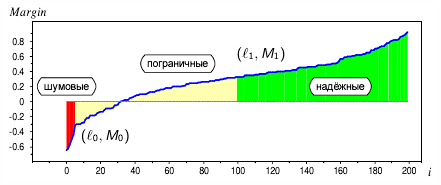
\includegraphics[width=15cm]{images/item_classes.png}

Не будем трогать те объекты, которые мы изначально классифицируем, как шумовые. \\
Тогда в результате применения ComBoost мы стремимся к тому, чтобы привести все оставшиеся объекты к надёжным, то есть привести эту кривую к таковой у бустинга. \\
Значит, естественно будет обучаться на тех объектах, что лежат в промежутке $[l_0, l_1]$ или же по отступам: $[M_0, M_1]$. \\
    
\textbf{Принцип максимизации и выравнивания отступов.}\
Получаем два случая, когда нам не нужно обучать $b_t$ на объекте $x_i$: \\
\begin{itemize}
    \item $M_{i,t-1} < M_0, i<l_0$, то есть объект шумовой.
    \item $M_{i,t-1} > M_1, i>l_1$, то есть объект надежно классифицируется.
\end{itemize}
    
Тогда, в отличие от бэггинга - мы возьмём нашу обучающую выборку не случайно, а по принципу, описанному выше. \\
    
\subsection{Алгоритм ComBoost}

Теперь, учитывая предыдущие выкладки, можно построить алгоритм:
\begin{enumerate}
    \item Инициализация. \\
    Выберем лучший из базовых алгоритмов $b_1$ по критерию качества и сгенерируем отступы $M_i = y_ib_1(x_i), i=1,\dots,l$. Для всех базовых алгоритмов, кроме выбранного, будем выполнять следующий шаг.
    \item Шаг алгоритма. \\
    Упорядочиваем выборку по возрастанию отступов. Обучим модели на множествах значимых объектов. А как строить эти множества значимых объектов? Будем проходить объемы обучающей выборки между минимальным - $l_1$ и максимальным - $l_2$ с некоторым шагом $\Delta l$, которые являются параметрами алгоритма: $U_t = \{x_i \in X^l : l_0 \leq i \leq k\}, k \in \{l1, \dots, l2\}$. \\
    Из полученных алгоритмов $b_{tk}$ выберем лучший по критерию $Q$: $b_t \in \{b_{tk}\}$, обновим отступы: $M_i = M_i + y_i b_t(x_i)$. Опционально можно изменить параметры $l_0, l_1$ и шаг в построении множеств значимых объектов.
    \item Окончание алгоритма \\
    Будем продолжать инкрементно улучшать набор базовых алгоритмов, пока критерий качества существенно улучшается.
    Таким образом мы получаем последовательность $b_1, \dots b_T$, составляющую итоговый ансамбль.
\end{enumerate}
    
Таким образом мы получаем алгоритм, который очень схож с бустингом и в значительной степени использует идеи бэггинга. \\
    
\subsection{Задачи}
    
\begin{enumerate}
    \item В шаге алгоритма ComBoost построение нового базового алгоритма происходит на подвыборках $U_t$, заходящих за границу $l_1$, которая определяет Надёжно классифицируемые объекты. Зачем это нужно?
        
    Ответ: Такой подход заимствован из инкрементного обучения, он позволяет нам улучшить уверенность модели на граничных случаях и её общую стабильность. В контексте ComBoost он так-же способствует разнообразию полученных базовых алгоритмов.
    
    \item Как можно перенести ComBoost на задачу о многоклассовой классификации?
        
    Ответ: Композицией наших алгоритмов можно взять простое голосование - каждый базовый алгоритм $b_{yt}$ голосует за свой класс $y$, то есть является бинарным классификатором. \\
    $a(x)=arg\max_{y\in Y}\Gamma_y(x)$, где $\Gamma_y(x) = \frac{1}{|T_y|}\sum_{t\in T_y}b_{yt}(x)$. \\
    Сам алгоритм изменится лишь в двух моментах: \\
    \begin{itemize}
        \item Отступ $M_i$ теперь считаем как максимум между правильным классом и произвольным другим. Тогда, если отступ отрицательный - ошибка есть, иначе - нет.
        \item Придётся решать, за какой из базовых классов мы хотим строить новый базовый алгоритм.
    \end{itemize}
    
    \item В чём проявляются идеи бэггинга и бустинга в алгоритме ComBoost?
    
    Ответ: От бустинга алгоритм берёт обучение по одному базовому алгоритму в строгой последовательности, а от бэггинга - обучение по подвыборкам.
\end{enumerate}


\section*{Теория и применение метода AnyBoost. Практические и продуктовые задачи с использованием AnyBoost. Сравнение AdaBoost и AnyBoost}
\subsection*{Введение}
Метод AnyBoost представляет собой обобщение алгоритмов бустинга, таких как AdaBoost, и направлен на последовательное построение композиции базовых алгоритмов для улучшения качества моделей машинного обучения. Его применение особенно полезно в задачах классификации и регрессии, где требуется минимизировать число ошибок или максимизировать отступы на обучающей выборке. Методика AnyBoost включает оптимизацию функций потерь и использование подхода прямой максимизации отступов, что делает её гибким и мощным инструментом для построения сложных моделей.

Метод AnyBoost возник из необходимости преодоления ограничений традиционных алгоритмов бустинга, таких как AdaBoost. Последние обладают высокой чувствительностью к выбросам и требуют значительных объемов данных. В отличие от этого, AnyBoost расширяет возможности работы с функциями потерь и предоставляет механизмы для оптимизации отступов, что позволяет использовать более широкий класс базовых алгоритмов. Это делает его универсальным решением для задач, требующих высокой точности и гибкости при построении моделей.

\subsection*{План}

\begin{itemize}
    \item \textbf{Предыстория и основы бустинга}
    \begin{itemize}
        \item Краткое описание теории бустинга
        \item Проблемы и ограничения стандартных методов (например, AdaBoost)
    \end{itemize}
    \item \textbf{Основы метода AnyBoost}
    \item \textbf{Научно-исследовательские и бизнес задачи и их решение}
\end{itemize}

\section*{Определение композиции}

\begin{itemize}
    \item $X^\ell = (x_i, y_i)_{i=1}^\ell \subset X \times Y$ — обучающая выборка, $y_i = y^*(x_i)$;
    \item $a(x) = C(b(x))$ — алгоритм, где
    \begin{itemize}
        \item $b: X \rightarrow R$ — базовый алгоритм (алгоритмический оператор),
        \item $C: R \rightarrow Y$ — решающее правило,
        \item $R$ — пространство оценок;
    \end{itemize}
\end{itemize}

\subsection*{Определение}
Композиция базовых алгоритмов $b_1, \ldots, b_T$

\[ a(x) = C(F(b_1(x), \ldots, b_T(x))), \]

где $F: R^T \rightarrow R$ — корректирующая операция.

\subsection*{Зачем вводится $R$?}
В задачах классификации множество отображений $\{F : R^T \rightarrow R\}$ существенно шире, чем $\{F : Y^T \rightarrow Y\}$.

\section*{Примеры пространств оценок и решающих правил}

\begin{itemize}
    \item \textbf{Пример 1}: классификация на 2 класса, $Y = \{-1, +1\}$:
    \[
    a(x) = \text{sign}(b(x)),
    \]
    где $R = \mathbb{R}$, $b: X \rightarrow \mathbb{R}$, $C(b) \equiv \text{sign}(b)$.
    
    \item \textbf{Пример 2}: классификация на $M$ классов $Y = \{1, \ldots, M\}$:
    \[
    a(x) = \arg \max_{y \in Y} b_y(x),
    \]
    где $R = \mathbb{R}^M$, $b: X \rightarrow \mathbb{R}^M$, $C(b_1, \ldots, b_M) \equiv \arg \max_{y \in Y} b_y$.
    
    \item \textbf{Пример 3}: регрессия, $Y = R = \mathbb{R}$:
    \[
    C(b) \equiv b
    \]
    — решающее правило не нужно.
\end{itemize}

\section*{Примеры корректирующих операций}

\begin{itemize}
    \item \textbf{Пример 1}: Простое голосование (Simple Voting):
    \[
    F(b_1(x), \ldots, b_T(x)) = \frac{1}{T} \sum_{t=1}^T b_t(x), \quad x \in X.
    \]

    \item \textbf{Пример 2}: Взвешенное голосование (Weighted Voting):
    \[
    F(b_1(x), \ldots, b_T(x)) = \sum_{t=1}^T \alpha_t b_t(x), \quad x \in X, \quad \alpha_t \in \mathbb{R}.
    \]

    \item \textbf{Пример 3}: Смешение алгоритмов (Mixture of Experts):
    \[
    F(b_1(x), \ldots, b_T(x)) = \sum_{t=1}^T g_t(x) b_t(x), \quad x \in X, \quad g_t: X \rightarrow \mathbb{R}.
    \]
\end{itemize}

\section*{Последовательное обучение композиции}

Функционал качества базового алгоритма, \(\mathcal{L}\) — функция потерь:

\[
Q(b, X^\ell) = \sum_{i=1}^\ell \mathcal{L}(b(x_i), y_i).
\]

Итерационный процесс:

\[
b_1 = \arg \min_{b} Q(b, X^\ell); \quad \tag{1}
\]

\[
b_2 = \arg \min_{b, F} Q(F(b_1, b), X^\ell);
\]

\[
\ldots
\]

\[
b_t = \arg \min_{b, F} Q(F(b_1, \ldots, b_{t-1}, b), X^\ell). \quad \tag{2}
\]

Идея: Свести задачу (2) к стандартной (1) с весами объектов и, возможно, с другой функцией потерь:

\[
b_t = \arg \min_{b} \sum_{i=1}^\ell w_i \tilde{\mathcal{L}}(b(x_i), y_i).
\]

\section*{Бустинг для задачи классификации с двумя классами}

Возьмём \( Y = \{\pm1\} \), \( b_t: X \rightarrow \{-1, 0, +1\} \), \( C(b) = \text{sign}(b) \).
\( b_t(x) = 0 \) — отказ (лучше промолчать, чем соврать).

Взвешенное голосование:

\[
a(x) = \text{sign}\left(\sum_{t=1}^T \alpha_t b_t(x)\right), \quad x \in X.
\]

Функционал качества композиции — число ошибок на \( X^\ell \):

\[
Q_T = \sum_{i=1}^\ell \left[ y_i \sum_{t=1}^T \alpha_t b_t(x_i) < 0 \right].
\]

Две основные эвристики бустинга:
\begin{itemize}
    \item фиксация \(\alpha_1 b_1(x), \ldots, \alpha_{t-1} b_{t-1}(x)\) при добавлении \(\alpha_t b_t(x)\);
    \item гладкая аппроксимация пороговой функции потерь \([M \leq 0]\).
\end{itemize}
\section*{Вопрос: Привести примеры аппроксимаций пороговой функции потерь}
\section*{Решение:}
\subsection*{Гладкие аппроксимации пороговой функции потерь}
\[
E(M) = e^{-M} \text{ — экспоненциальная (AdaBoost);}
\]

\[
L(M) = \log_2(1 + e^{-M}) \text{ — логарифмическая (LogitBoost);}
\]

\[
Q(M) = (1 - M)^2 \text{ — квадратичная (GentleBoost);}
\]

\[
G(M) = \exp\left(-cM(M + s)\right) \text{ — гауссовская (BrownBoost);}
\]

\[
S(M) = 2(1 + e^{M})^{-1} \text{ — сигмоидная;}
\]

\[
V(M) = (1 - M)_+ \text{ — кусочно-линейная (из SVM);}
\]

\section*{Обозначения для док-ва основной теоремы бустинга}

Оценка функционала качества \(Q_T\) сверху:

\[
Q_T \leq \widetilde{Q}_T = \sum_{i=1}^\ell \exp\left(-y_i \sum_{t=1}^{T-1} \alpha_t b_t(x_i)\right) \exp\left(-y_i \alpha_T b_T(x_i)\right)
\]

\[
\phantom{Q_T \leq \widetilde{Q}_T} = \underbrace{\sum_{i=1}^\ell \frac{w_i}{\sum_{j=1}^\ell w_j}}_{\widetilde{W}^\ell = (\widetilde{w}_1, \ldots, \widetilde{w}_\ell), \, \widetilde{w}_i = w_i / \sum_{j=1}^\ell w_j}.
\]

Взвешенное число ошибочных (negative) и правильных (positive) классификаций при векторе весов \(U^\ell = (u_1, \ldots, u_\ell)\):

\[
N(b, U^\ell) = \sum_{i=1}^\ell u_i [b(x_i) = -y_i]; \quad P(b, U^\ell) = \sum_{i=1}^\ell u_i [b(x_i) = y_i].
\]

\(1 - N - P\) — взвешенное число отказов от классификации.

\section*{Теоретическая задача}
Сформулировать основную теорему бустинга (достаточно для AdaBoost) и привести док-во этой теоремы. Сформулировать следствие. Рассказать про AdaBoost и AnyBoost

\section*{Решение}
\section*{Основная теорема бустинга (для AdaBoost)}
Пусть B — достаточно богатое семейство базовых алгоритмов

Пусть для любого нормированного вектора весов \(U^\ell\) существует алгоритм \(b \in B\), классифицирующий выборку хотя бы немного лучше, чем наугад: \(P(b; U^\ell) > N(b; U^\ell)\).

Тогда минимум функционала \(\widetilde{Q}_T\) достигается при

\[
b_T = \arg \max_{b \in B} \sqrt{P(b; \widetilde{W}^\ell)} - \sqrt{N(b; \widetilde{W}^\ell)}.
\]

\[
\alpha_T = \frac{1}{2} \ln \frac{P(b_T; \widetilde{W}^\ell)}{N(b_T; \widetilde{W}^\ell)}.
\]

\section*{Доказательство}

Воспользуемся тождеством \(\forall \alpha \in \mathbb{R}, \, \forall b \in \{-1, 0, +1\}\):

\[
e^{-\alpha b} = e^{-\alpha}[b = 1] + e^{\alpha}[b = -1] + [b = 0].
\]

Положим для краткости \(\alpha = \alpha_T\) и \(b_i = b_T(x_i)\). Тогда

\[
\widetilde{Q}_T = \left(e^{-\alpha} \sum_{i=1}^\ell \widetilde{w}_i[b_i = y_i] + e^{\alpha} \sum_{i=1}^\ell \widetilde{w}_i[b_i = -y_i] + \sum_{i=1}^\ell \widetilde{w}_i[b_i = 0]\right) \sum_{i=1}^\ell w_i
\]

\[
= \underbrace{e^{-\alpha} P + e^{\alpha} N}_{P \; N} + (1 - P - N) \widetilde{Q}_{T-1} \rightarrow \min_{\alpha, b}.
\]

\[
\frac{\partial}{\partial \alpha} \widetilde{Q}_T = (-e^{-\alpha} P + e^{\alpha} N) \widetilde{Q}_{T-1} = 0 \implies e^{-\alpha} P = e^{\alpha} N \implies e^{2\alpha} = \frac{P}{N}.
\]

Получили требуемое:

\[
\alpha_T = \frac{1}{2} \ln \frac{P}{N}.
\]

Подставим оптимальное значение \(\alpha = \frac{1}{2} \ln \frac{P}{N}\) обратно в \(\widetilde{Q}_T\):

\[
\widetilde{Q}_T = (e^{-\alpha} P + e^{\alpha} N + (1 - P - N)) \widetilde{Q}_{T-1} = 
\]

\[
= \left(1 + \sqrt{\frac{N}{P}} P + \sqrt{\frac{P}{N}} N - P - N\right) \widetilde{Q}_{T-1} = 
\]

\[
= \left(1 - (\sqrt{P} - \sqrt{N})^2\right) \widetilde{Q}_{T-1} \rightarrow \min_b.
\]

Поскольку \(\widetilde{Q}_{T-1}\) не зависит от \(\alpha_T\) и \(b_T\), минимизация \(\widetilde{Q}_T\) эквивалентна либо максимизации \(\sqrt{P} - \sqrt{N}\) при \(P > N\), либо максимизации \(\sqrt{N} - \sqrt{P}\) при \(P < N\), однако второй случай исключён условием теоремы.

Получили

\[
b_T = \arg \max_b \sqrt{P} - \sqrt{N}.
\]

Теорема доказана.


\section*{Следствие. Классический вариант AdaBoost}

Пусть отказов нет, $b_t : X \to \{ \pm 1 \}$. Тогда $P = 1 - N$.
\subsection*{Вопрос: формулировка теормы Freund, Schapire, 1995}
\subsection*{Теорема (Freund, Schapire, 1995)}

Пусть для любого нормированного вектора весов $U^\ell$ существует алгоритм $b \in B$, классифицирующий выборку хотя бы немного лучше, чем наугад: $N(b; U^\ell) < \frac{1}{2}$.

Тогда минимум функционала $\tilde{Q}_T$ достигается при

\[
b_T = \arg \min_{b \in B} N(b; W^\ell).
\]

\[
\alpha_T = \frac{1}{2} \ln \frac{1 - N(b_T; \tilde{W}^\ell)}{N(b_T; \tilde{W}^\ell)}
\]


\section*{Алгоритм AdaBoost}

\textbf{Вход:} обучающая выборка $X^\ell$, параметр $T$;\\
\textbf{Выход:} базовые алгоритмы и их веса $\alpha_t b_t$, $t = 1, \ldots, T$;

\begin{enumerate}
    \item инициализировать веса объектов:
    \[
    w_i := \frac{1}{\ell}, \quad i = 1, \ldots, \ell;
    \]
    \item \textbf{для всех} $t = 1, \ldots, T$
    \begin{enumerate}
        \item обучить базовый алгоритм:
        \[
        b_t := \arg \min_b N(b; W^\ell);
        \]
        \item 
        \[
        \alpha_t := \frac{1}{2} \ln \frac{1 - N(b_t; W^\ell)}{N(b_t; W^\ell)};
        \]
        \item обновить веса объектов:
        \[
        w_i := w_i \exp(-\alpha_t y_i b_t(x_i)), \quad i = 1, \ldots, \ell;
        \]
        \item нормировать веса объектов:
        \[
        w_0 := \sum_{j=1}^{\ell} w_j;
        \]
        \[
        w_i := w_i / w_0, \quad i = 1, \ldots, \ell;
        \]
    \end{enumerate}
\end{enumerate}

\section*{Недостатки AdaBoost}

\begin{itemize}
    \item Чрезмерная чувствительность к выбросам из-за $e^{-M}$.
    \item AdaBoost строит «чёрные ящики». Громоздкие композиции из сотен алгоритмов не интерпретируемы.
    \item Не удаётся строить короткие композиции из «сильных» алгоритмов типа SVM (только длинные из слабых).
    \item Требуются достаточно большие обучающие выборки (бэггинг обходится более короткими — см. далее).
\end{itemize}

Способы устранения:
\begin{itemize}
    \item Другие аппроксимации пороговой функции потерь.
    \item Непрерывные вещественные базовые алгоритмы $b_t: X \to \mathbb{R}$.
    \item Явная оптимизация отступов (ComBoost может строить короткие композиции из хороших алгоритмов).
\end{itemize}

\section*{Обобщение базового классификатора и функции потерь}

Возьмём $Y = \{\pm 1\}$, $b_t : X \to \mathbb{R}$, $C(b) = \text{sign}(b)$;\\
$\mathcal{L}(M)$ — функция потерь, гладкая функция отступа $M$;

\[
M_T(x_i) = y_i \sum_{t=1}^{T} \alpha_t b_t(x_i) \text{ — отступ композиции на объекте } x_i;
\]

Оценка сверху для числа ошибок композиции:

\[
Q_T \leq \tilde{Q}_T = \sum_{i=1}^{\ell} \mathcal{L}(M_{T-1}(x_i) + \alpha y_i b(x_i)) \to \min_{\alpha, b}.
\]

Линеаризация функции потерь по $\alpha$ в окрестности $\alpha = 0$:

\[
\tilde{Q}_T \approx \sum_{i=1}^{\ell} \mathcal{L}(M_{T-1}(x_i)) - \alpha \sum_{i=1}^{\ell} -\mathcal{L}'(M_{T-1}(x_i)) y_i b(x_i) \to \min_{b},
\]
где $w_i$ — веса объектов.

\section*{Принцип явной максимизации отступов}

Минимизация линеаризованного $\tilde{Q}_T$ при фиксированном $\alpha$

\[
\tilde{Q}_T \approx \sum_{i=1}^{\ell} \mathcal{L}(M_{T-1}(x_i)) - \alpha \sum_{i=1}^{\ell} w_i y_i b(x_i) \to \min_{b}.
\]

приводит к принципу \textit{явной максимизации отступов} (direct optimization of margin, DOOM):

\[
\sum_{i=1}^{\ell} w_i y_i b(x_i) \to \max_{b}.
\]

Затем $\alpha$ определяется путём одномерной минимизации $\tilde{Q}_T$.

Итерации этих двух шагов приводят к алгоритму AnyBoost.

\textit{Замечание.} AnyBoost переходит в AdaBoost в частном случае, при $b_t : X \to \{-1, 0, +1\}$ и $\mathcal{L}(M) = e^{-M}$.


\section*{Алгоритм AnyBoost}

\textbf{Вход:} обучающая выборка $X^\ell$, параметр $T$;\\
\textbf{Выход:} базовые алгоритмы и их веса $\alpha_t b_t$, $t = 1, \ldots, T$;

\begin{enumerate}
    \item инициализировать отступы: 
    \[
    M_i := 0, \quad i = 1, \ldots, \ell;
    \]
    \item \textbf{для всех} $t = 1, \ldots, T$
    \begin{enumerate}
        \item вычислить веса объектов:
        \[
        w_i = -\mathcal{L}'(M_i), \quad i = 1, \ldots, \ell;
        \]
        \item обучить базовый алгоритм согласно принципу DOOM:
        \[
        b_t := \arg \max_{b} \sum_{i=1}^{\ell} w_i y_i b(x_i);
        \]
        \item решить задачу одномерной минимизации:
        \[
        \alpha_t := \arg \min_{\alpha > 0} \sum_{i=1}^{\ell} \mathcal{L}(M_i + \alpha b_t(x_i) y_i);
        \]
        \item обновить значения отступов:
        \[
        M_i := M_i + \alpha_t b_t(x_i) y_i, \quad i = 1, \ldots, \ell;
        \]
    \end{enumerate}
\end{enumerate}

\section*{Исследовательская задача}
\subsection*{Постановка задачи}
\textbf{Цель:} Исследовать, как различная функциональная гибкость в обработке ошибок может повлиять на точность классификации. Сравнить модели AdaBoost и AnyBoost для определения, какая из них обеспечивает более высокую точность за счет использования различных функций потерь.

\textbf{Проблема:} Сравнить влияние выбора функции потерь на производительность моделей и определить, может ли AnyBoost предложить лучшее решение, чем стандартный AdaBoost.

\subsection*{Формализация задачи}

- Задача классификации с бинарными метками: $y \in \{0, 1\}$.
- Датасет $X = \{x_1, x_2, \ldots, x_n\}$ с известными метками.
- Сравнить точность моделей $f_{AdaBoost}(x)$ и $f_{AnyBoost}(x)$.

\section*{Эксперимент}

\subsection*{Датасет}
Используется открытый датасет (например, из UCI Machine Learning Repository) или синтетический набор данных, в котором сложна линейная классификация.

\subsection*{Модели}

\textbf{AdaBoost:}
\begin{itemize}
    \item Использовать стандартную реализацию AdaBoost с решающими пнями как базовыми алгоритмами.
    \item Применять экспоненциальную функцию потерь.
\end{itemize}

\textbf{AnyBoost:}
\begin{itemize}
    \item Использовать те же базовые алгоритмы, но протестировать несколько функций потерь, включая:
    \begin{itemize}
        \item Экспоненциальную (как в AdaBoost для сравнения).
        \item Логарифмическую (log loss).
        \item Квадратичную (quadratic loss).
    \end{itemize}
\end{itemize}

\subsection*{Оценка}
\begin{itemize}
    \item Разделить данные на обучающую, валидационную и тестовую выборки.
    \item Обучить обе модели.
    \item Оценить с использованием метрик точности (accuracy), F1-score и AUC-ROC.
\end{itemize}

\subsection*{Гипотеза и тестирование}
\begin{itemize}
    \item Гипотеза: AnyBoost с адаптацией к функции потерь, отличной от экспоненциальной, покажет лучшие результаты в задачах, где ошибки влияют по-разному.
    \item Тестирование с использованием статистического анализа значимости различий в производительности (например, тест Стьюдента).
\end{itemize}

\subsection*{Результаты и выводы}

- Если $f_{AnyBoost}(x)$ показывает значительное улучшение по сравнению с $f_{AdaBoost}(x)$, это свидетельствует о том, что функциональная гибкость AnyBoost позволяет лучше адаптироваться к свойствам датасета.
- Функциональная гибкость позволяет лучше справляться с различными типами данных и адаптироваться к специфичным особенностям задач.

\subsection*{Дальнейшие направления}
Изучение AnyBoost на более широком классе данных и функций потерь, применение в мультиклассовых задачах и оценка метрик устойчивости модели на данных с шумом.


\section*{Формализованные задачи с использованием AnyBoost}

\subsection*{Задача 1: Прогнозирование оборудования на производстве}

\textbf{Проблема:} Необходимо предсказать поломки производственного оборудования для предотвращения простоев.

\textbf{Формализация:} 
Рассмотрим набор данных $X = \{x_1, x_2, \ldots, x_n\}$, где $x_i$ — вектор признаков, таких как вибрации, температура и давление. Цель — обучить модель $f(x)$, предсказывающую вероятность поломки $y \in \{0, 1\}$.

\textbf{Пример:} 
Пусть данные собираются каждые 10 минут, а за месяц получено $n = 10\,000$ записей. Средние значения: вибрация = $0.02$, температура = $50^\circ C$, давление = $5$ Бар.

\textbf{Решение с AnyBoost:}
\begin{itemize}
    \item \textbf{Сбор данных:} Собрать 10\,000 записей, включая следующие параметры: вибрация, температура и давление.
    \item \textbf{Обработка данных:} Нормализовать данные, чтобы значения признаков лежали в диапазоне [0, 1].
    \item \textbf{Обучение модели:} Использовать AnyBoost с функцией потерь, подходящей для дисбалансированных данных, например, "focal loss".
    \item \textbf{Настройка параметров:} Количество базовых алгоритмов (деревьев решений) = 100; max\_depth = 5.
    \item \textbf{Оценка качества:} Тестировать модель на 2\,000 новых записей, достигая F1-score = 0.85.
    \item \textbf{Внедрение и мониторинг:} Внедрить модель для прогноза в реальном времени, настроить систему оповещения при превышении вероятности поломки 0.7.
\end{itemize}

\textbf{Пример последовательного предсказания:}
\begin{itemize}
    \item Рассмотрим вектор $x_{test} = [0.015, 45, 4.5]$.
    \item Этап 1: Запуск базового алгоритма №1.
        \begin{itemize}
            \item Выход: предсказание вероятности = 0.4.
            \item Обновление весов: увеличиваются веса ошибочно классифицированных примеров.
        \end{itemize}
    \item Этап 2: Запуск базового алгоритма №2 с обновленными весами.
        \begin{itemize}
            \item Выход: предсказание вероятности = 0.6.
            \item Снова корректировка весов.
        \end{itemize}
    \item Итерация на последнем базовом алгоритме №100.
        \begin{itemize}
            \item Итоговое предсказание после агрегирования всех вероятностей = 0.72, что указывает на высокую вероятность поломки.
        \end{itemize}
\end{itemize}


\subsection*{Задача 2: Прогнозирование риска сердечно-сосудистых заболеваний}

\textbf{Проблема:} Предсказать риск сердечно-сосудистых заболеваний для раннего вмешательства.

\textbf{Формализация:} 
Пусть $X = \{x_1, x_2, \ldots, x_n\}$ — набор данных пациентов с признаками, такими как возраст, ИМТ и уровень холестерина. Цель — обучить модель $g(x)$ для предсказания риска $y \in [0, 1]$.

\textbf{Пример:} 
Пациенты: $n = 5\,000$. Средний возраст = 45, средний ИМТ = 27, средний уровень холестерина = 210 мг/дл.

\textbf{Решение с AnyBoost:}
\begin{itemize}
    \item \textbf{Сбор данных:} Использовать медицинские данные для 5\,000 пациентов. 
    \item \textbf{Обработка данных:} Нормализовать индексы массы тела и ур. холестерина, отсеять пропущенные данные.
    \item \textbf{Обучение модели:} Обучить модель AnyBoost с функцией потерь, минимизирующей ошибочные предсказания высокого риска, например, "log loss".
    \item \textbf{Настройка параметров:} Количество базовых алгоритмов = 150; learning\_rate = 0.05.
    \item \textbf{Оценка качества:} Достичь AUC-ROC = 0.92 на тестовой выборке из 1\,000 пациентов.
    \item \textbf{Внедрение в практику:} Обеспечить использование модели в клиниках для выявления пациентов с риском $\geq 0.8$ и направления их на дополнительные обследования.
\end{itemize}

\textbf{Пример последовательного предсказания:}
\begin{itemize}
    \item Рассмотрим данные пациента $x_{patient} = [50, 29, 240]$, где возраст = 50, ИМТ = 29, холестерин = 240.
    \item Этап 1: Базовый алгоритм №1.
        \begin{itemize}
            \item Вероятность риска = 0.65.
        \end{itemize}
    \item Этап 2: Базовый алгоритм №2.
        \begin{itemize}
            \item Вероятность обновляется до 0.7.
        \end{itemize}
    \item На 150-м базовом алгоритме.
        \begin{itemize}
            \item Итоговое предсказание = 0.83, указывающее на высокий риск и необходимость дополнительных мер.
        \end{itemize}
\end{itemize}


\subsection*{Задача 3: Кластеризация экспериментов для анализа научных данных}

\textbf{Проблема:} Классифицировать эксперименты на группы для эффективного анализа.

\textbf{Формализация:} 
Имеется набор данных $\{X_1, X_2, \ldots, X_m\}$, где каждый $X_i$ — набор параметров эксперимента. Цель — разбить на кластеры $C_1, C_2, \ldots, C_k$, минимизируя внутрикластерные расстояния.

\textbf{Пример:} 
Эксперименты: $m = 500$. Средние параметры: температура = $25^\circ C$, концентрация реагента = 0.01 М, скорость реакции = 5 м/ч.

\textbf{Решение с AnyBoost:}
\begin{itemize}
    \item \textbf{Сбор данных:} Собрать и стандартизировать данные 500 экспериментов.
    \item \textbf{Обработка данных:} Провести предварительный анализ на выбросы и отклонения.
    \item \textbf{Обучение модели:} Использовать AnyBoost для обнаружения паттернов и аномалий, используя комбинацию "k-means" и AnyBoost.
    \item \textbf{Настройка параметров:} Количество кластеров $k = 5$; провести оптимизацию с использованием метода "elbow method".
    \item \textbf{Оценка результата:} Оценить качество кластеризации с помощью индекса силуэта, добиться значения > 0.75.
    \item \textbf{Интерпретация результатов:} Представить результаты исследователям для анализа и выявления закономерностей, что может помочь в оптимизации экспериментов.
\end{itemize}
\textbf{Пример последовательной кластеризации:}
\begin{itemize}
    \item Рассмотрим эксперимент $x_{exp} = [25, 0.005, 6]$, где температура = $25^\circ C$, концентрация = 0.005 М, скорость = 6 м/ч.
    \item Этап 1: Инициализация кластеризации с базовым алгоритмом №1.
        \begin{itemize}
            \item Предварительная кластерная группа — Cluster 2.
        \end{itemize}
    \item Этап 2: Базовый алгоритм №2 с коррекцией на фоне других экспериментов.
        \begin{itemize}
            \item Изменение вероятности принадлежности к Cluster 2, новое предсказание = Cluster 3.
        \end{itemize}
    \item Итоговое решение после алгоритма №50.
        \begin{itemize}
            \item Окончательное отнесение к Cluster 3 с индексом соответствует высокой схожести с параметрами других экспериментов в этом кластере.
        \end{itemize}
\end{itemize}


\section*{RandomBoosting}

RandomBoosting - метод бустинга, в котором используется случайность при построении решающих деревьев. Алгоритм во многом схож с классическим градиентным бустингом, однако с добавляением случайной глубины деревьев, что позволяет улучшить эффективность модели.

\subsection*{Зачем изучать RandomBoosting}
\begin{enumerate}
    \item \mathbf{Борьба с переобучением.} Ввод случайности в процесс построения деревьев помогает уменьшить корреляцию между деревьями в ансамбле.
    \item \mathbf{Ускорение вычислений.} Модель использует более простые деревья, поэтому сам процесс обучения ускоряется. 
\end{enumerate}

\subsection*{Регрессионные деревья}
\mathbf{Определение.} Регресионные деревья - это модели, которые можно описать следующим рекурсивным правилом (по сути это алгоритм CART~--- Classification And Regression Tree):
\begin{enumerate}
    \item Дерево сначала строится до максимально возможного размера.
    \item Затем дерево уменьшается до оптимального размера (фаза "pruning").
\end{enumerate}

Пусть дан набор данных $\mathcal{L} = \{(x_i, y_i)\}_{i = 1}^N$. Зафиксируем элемент $x_j$, ещё называемый "предиктором", и элемент $s$~--- значение распределения, такие что:
$$R_1 = \{x | x_j \leq s\}, R_2=\{x | x_j > s\}$$.

Алгоритм CART вычисляет среднее значение овтета, при помощи минимизации функции квадратов ошибок (т.н. SSE). На выходе имеем модель в форме дерева: $\{t_1, ...,t_T\}$~--- узлы дерева, а $T$~--- количество листьев. 

Теперь получим из этого дерева прогноз $\hat{f}(x)=\bar{y}_j$, где $y_j$~--- среднее значение переменной в узле $t_j$. Или верна следующая запись:

\begin{center}   
$\bar{f}(x) = \sum_{t=1}^T \mathbf{1}(x \in t_j)\gamma_j$, где $\gamma_j$~---среднее значение ответа в узле $t_j$.
\end{center}

Из-за особенностей работы алгоритма CART для построение дерева максимально возможной глубины, есть большой риск переобучения модели. Чтобы избежать этой проблемы, деревья нужно обрезать (применить операцию "pruning").

Однако данный подход имеет проблему, так как за незначительными разрывами могут следовать "значительные". Поэтому был разработан альтернативный алгоритм:
\begin{enumerate}
    \item Дерево сначала строится до максимально возможного размера.
    \item Уменьшить дерево с помощью обратного пошагового метода обрезки ("pruning") на основе некоторого критерия (можно использовать кросс-валидацию - CV).
\end{enumerate}

По итогу, благодаря этому подходу, получается метод, близкий к "готовому", не требующий дополнительной настройки, поэтому имеем следующие преимущества данного алгоритма:
\begin{enumerate}
    \item Деревья могут работать с пропущенными значениями при помощи вспомогательных разбиений
    \item Деревья не восприимчивы к выбросам среди признаков
    \item Деревья устойчивы к шуму в данных
    \item Деревья устойчивы к строго монотонным преобразованиям признаков
\end{enumerate}

Однако, есть и минусы: деревья нестабильны, так как разбиения в родительском узле влияют на разбиением в узлах-потомках.

\subsection*{Параллельные ансамбли}
Для решения проблемы нестабильности CART было предложено решение, которое улучшает предсказательную способность по сравнению с одним регрессионным деревом. Модель использует так называемый метод бутстраппинга и агрегации (или одним словом - bagging). 

Назовём бутстрэп выборкой $\mathcal{B}_b$, $b=1,...,B$, независимо (с возвращением) извлекающуюся из выборки $\mathcal{L}$. Для каждой бутстрэп-выборки построим регрессионные деревья, как в прошлом пункте $\Rightarrow$ получим последовательность обучающих моделей $\{f_b\}_{b=1}^B$. Тогда итоговая модель может быть получена следующим образом:
$$\hat{f}_{bagging}(x) = \frac{1}{B}\sum_{b=1}^B \hat{f}_b(x)$$

Преимущество бэггинга заключаются в том, что он усредняет нестабильные деревья, возвращая стабильность предсказаниям ансамбля, и как следствие, повышается предсказательная способность.

\subsection*{Последовательные ансамбли}
В бэггинге модели строятся параллельно и независимо, но в бустинге они обучаются последовательно. Бустинг строит последовательный ансамбль, где базовые процедуры создаются поэтапно, что приводит к тому, что они перестают быть независимыми.

Вспомним идею AdaBoost: выделяется два ключевых аспекта бустинга:
\begin{enumerate}
    \item Каждый элемент обучается на уникальной части данных, получая измененную версию исходных данных в качестве входных 
    \item Изменения зависят от предыдущих моделей
\end{enumerate}

Идея заключается в том, чтобы сочетать эти два концепта. Более формально, пусть $y$~--- случайный выход и случайный вектор входных данных $x$.
Хотим найти приближении функции $\hat{F}$ к функции $F^*$: $x$ $\rightarrow$ $y$ с минимальными ожидаемыми потерями.

Введём $F(x, \theta)$, где $\theta$~--- параметр.

Построим задачу оптимизации:
$$F(x, \alpha, \beta) = \sum_{m = 0}^M \alpha_m f(x, \beta_m)$$ где $f(x, \beta_m)$~--- простая параметризованная функция, а $\alpha$ и $\beta$~--- параметры.

Тогда задача оптимизации превращается в задачу оптимизации параметров:
$$\theta^* = \arg \min_{\theta} \mathbb{E}_{Y, X} [L(y, F(x, \theta)]$$
и $F^*(x)=F(x, \theta^*)$.

Итого, решаем эту задачу при помощи градиентного спуска, приближая $\theta^*$ шаг за шагом, начиная с оценки $\theta_0$. Итого, по итогу конечная оценка:
$$\hat{\theta} = \sum_{m=0}^M \theta_m$$

Итого, легко видеть, что помимо оценки $\theta_0$ важно рассматривать другие параметры задачи: количество шагов бустинга $M$ и длину шага.

\subsection*{Дополнительная случайность}
В бэггинге случайность снижает вариацию прогнозов, поэтому его производительность не сильно отлична от бустинга. По этой причине был предложен стохастический градиентный бустинг - своего рода гибрид бэггинга и бустинга, в которой на каждой итерации строится дерево на случайно подвыборке данных. На практике данный подход позволяет ускорить алгоритм и повысить точность прогноза.

\subsection*{$\mathbf{Random^2}$ Forests}
Одной из наиболее успешных примеров, использующих вышеописанную концепцию, является $Random^2$ Forest (или просто R2F).

R2F - это дополнение существующего метода случайных лесов (RF). Например, при одинаковых значениях для размера дерева, R2F более эффективен.

Пусть RF обучаются с максимальной глубиной дерева $d_{max}$, деревья в R2F имеют глубину $d$.

Тогда для RF количество разбиений $s$ для регрессивного дерева глубины $d_{max}$ равняется:
$$s_{RF}(d_{max})=l - 1 \leq 2^{d_{max}} - 1$$
где $l$~--- количество листьев.

Для R2F это иначе: дерево глубины $d$ растёт с вероятностью $P(D=d) = \frac{1}{d_{max}}$. Тогда количество разбиений можно оценить так:
$$s_{R2F}(d_{max})\leq\frac{1}{d_{max}} \sum_{d=1}^{d_max}\left(2d-1\right)$$

Или, приближая, получим примерную формулу для относительного числа разбиений:
$$s_{rel}(d_{max}) = \frac{s_{R2F}}{s_{RF}} \cong \frac{2}{d_{max}} \left(1 - \left(\frac{1}{2}\right)^{d_{max}}\right)$$

\subsection*{Random Boost}
Наконец, перейдём к Random Boost (RB). Метод аналогичен R2F: в RB рассматривается глубина $d$ как дискретная случайная равномерно распределённая величина. Если быть точным, на каждом шаге выбирается случайная глубина дерева $d \in [1, d_{max}]$.

Таким образом, получается последовательность деревьев с разной глубиной: $f_1(x, \beta_1, d_1),...,f_M(x, \beta_M, d_M)$.

Итого:
$$\hat{f}_{RB}(x)=\sum_{m=1}^M \alpha_m f_m(x, \beta_m, d_m)$$

Преимуществом RB является тот факт, что он оказывается более вычислительно эффективным, чем традиционные методы, при условии, что используются одинаковые значения для максимальной глубины дерева.

\subsection*{Задачи}

\textbf{Задача 1}:
Максимальная глубина деревьев в R2F составляет $d_{max} = 4$. Найти относительное число разбиений $s_{rel}(d_{max})$ для R2F по сравнению с RF.

\textbf{Решение:}
Мы знаем, что $s_{rel}(d_{max})\cong\frac{2 \left(1-\left(\frac{1}{2}\right)^{d_{max}}\right)}{d_{max}}$

$s_{rel}(4) \cong \frac{2 \cdot (1 - \frac{1}{16})}{4} = \frac{15}{32}$

\textbf{Задача 2}:
Использование случайной подвыборки размером 40\% уменьшает абсолютную ошибку градиентного бустинга на 11\%. Если начальная ошибка модели составляет 0.45, найдите уменьшенную ошибку при применении стохастического градиентного бустинга.

\textbf{Решение:}
\begin{center}    
Новая ошибка = Начальная ошибка $\cdot (1 - 0.11) = 0.45 \cdot 0.89 \cong 0.4$
\end{center}

\textbf{Задача 3}:
В R2F максимальная глубина деревьев $d_{max} = 5$. Найдите:
\begin{enumerate}
    \item P(D=3)
    \item Средняя глубина дерева
\end{enumerate}

\textbf{Решение:}
\begin{enumerate}
    \item 
    В R2F глубина равномерно распределена на интервале $[1, d_{max}]$.
    Тогда, $P(D=d) = \frac{1}{d_{max}} = \frac{1}{5}$

    \item 
    Распределение равномерное, тогда:

    $$\mathbb{E}(D) = \frac{1 + d_{max}}{2} = \frac{1 + 5}{2} = 3$$
\end{enumerate}


\section*{Стэкинг. Линейный стэкинг, взвешенный по признакам}

\subsection*{Введение}

Стэкинг (stacking) — это метод ансамблирования, который позволяет объединять предсказания нескольких моделей для получения более точного результата. В отличие от более простых подходов, таких как бэггинг или бустинг, стэкинг использует метамодель, которая обучается на выходах базовых моделей, чтобы улучшить качество финальных предсказаний.
\\
\\
Представьте голосование в жюри: разные судьи выносят свои оценки, но финальное решение принимается главным судьей, который учитывает сильные и слабые стороны каждого члена жюри. Стэкинг работает аналогично: базовые модели создают метапризнаки, а метамодель решает, как их комбинировать.

\subsection*{Классический стэкинг}


Основная идея классического стэкинга заключается в следующем:
\begin{enumerate}
    \item Данные разбиваются на \( k \)-фолдов (частей) для кросс-валидации.
    \item Для каждого фолда:
    \begin{enumerate}
        \item Базовые модели обучаются на данных из \( k-1 \) фолдов.
        \item На оставшемся \( k \)-м фолде вычисляются предсказания для объектов, которые формируют метапризнаки \( b_{tj}(x) \) для данного фолда.
    \end{enumerate}
    \item Для каждого объекта собираются предсказания базовых моделей, сделанные на разных фолдах. При необходимости они могут усредняться:
    \[
    b_t(x) = \frac{1}{k} \sum_{j=1}^k b_{tj}(x).
    \]
     где \( b_{tj}(x) \) \textemdash предсказания базовой модели на \( j \)-м фолде, а \( b_t(x) \) \textemdash итоговый метапризнак.
    \item На основе полученного набора метапризнаков и истинных меток обучается метамодель.
\end{enumerate}

Такой подход позволяет использовать полную информацию из данных, минимизируя риск переобучения. 



\subsection*{Линейный взвешенный стэкинг (Feature-Weighted Linear Stacking)}

Линейный взвешенный стэкинг расширяет классический стэкинг, добавляя возможность учитывать важность признаков через веса. Итоговое предсказание вычисляется как линейная комбинация метапризнаков с учетом весов:
\[
    b(x) = \sum_{t=1}^T \alpha_t b_t(x),
\]
где \( \alpha_t \) — веса моделей, которые зависят от признаков объекта через функции \( f_j(x) \):
\[
    \alpha_t(x) = \sum_{j=1}^L v_{tj} f_j(x).
\]
где \( v_{tj} \) \textemdash~обучаемые параметры.


Для оптимизации весов \( v_{tj} \) используется ридж-регрессия:
\[
Q(v) = \sum_{i=1}^\ell \left( \sum_{t=1}^T \sum_{j=1}^L v_{tj} f_j(x_i) b_t(x_i) - y_i \right)^2 + \frac{\lambda}{2} \sum_{t=1}^T \sum_{j=1}^L v_{tj}^2 \to \min_v.
\]
Метапризнаки \( f_j \) могут быть как фиксированными, так и обучаемыми (задача симметрична относительно \( b_t \) и \( f_j \)), что делает метод более гибким.

Линейный взвешенный стэкинг позволяет учитывать важность признаков объекта для предсказаний и улучшать качество модели.


\section*{Задачи}

\subsection*{Задача 1: Классический стэкинг}

Имеется выборка из 10 объектов, разбитая на 5 фолдов. Для объекта \( x_7 \) предсказания базовых моделей составляют:
\[
b_{t1}(x_7) = 0.8, \ b_{t2}(x_7) = 0.7, \ b_{t3}(x_7) = 0.9, \ b_{t4}(x_7) = 0.6, \ b_{t5}(x_7) = 0.85.
\]

Вычислите итоговый метапризнак \( b_t(x_7) \).
\\
\textbf{Решение:}
\[
b_t(x) = \frac{1}{k} \sum_{j=1}^k b_{tj}(x).
\]
\[
b_t(x_7) = \frac{1}{5} (0.8 + 0.7 + 0.9 + 0.6 + 0.85) = 0.77.
\]



\subsection*{Задача 2: Учет весов в метапризнаках}

Для объекта \( x \) весовые функции \( f_1(x) = 1 \) и \( f_2(x) = 2 \), а веса моделей:
\[
\alpha_1(x) = 0.5 f_1(x), \ \alpha_2(x) = 0.5 f_2(x).
\]
Предсказания моделей:
\[
b_1(x) = 0.7, \ b_2(x) = 0.9.
\]

Вычислите итоговое предсказание \( b(x) \).
\\
\textbf{Решение:}
\[
\alpha_1(x) = 0.5 \cdot 1 = 0.5, \ \alpha_2(x) = 0.5 \cdot 2 = 1.
\]
\[
b(x) = \alpha_1(x) b_1(x) + \alpha_2(x) b_2(x).
\]
\[
b(x) = 0.5 \cdot 0.7 + 1 \cdot 0.9 = 1.25.
\]



\subsection*{Задача 3: Моделирование обучения метамодели}

Даны метапризнаки, созданные на основе двух базовых моделей. Каждая строка представляет объект:
\[
\text{Объект 1: } b_1(x) = 0.8, \ b_2(x) = 0.6, \ y = 1.0,
\]
\[
\text{Объект 2: } b_1(x) = 0.4, \ b_2(x) = 0.7, \ y = 0.5,
\]
\[
\text{Объект 3: } b_1(x) = 0.6, \ b_2(x) = 0.8, \ y = 0.7.
\]

\textbf{Требуется:}
\begin{enumerate}
    \item Постройте линейную регрессию, обученную на метапризнаках $b_1(x)$ и $b_2(x)$, чтобы предсказать $y$.
    \item Найдите параметры регрессии ($\beta_1, \beta_2$).
    \item Сделайте прогноз для объекта с $b_1(x) = 0.7, \ b_2(x) = 0.5$.
\end{enumerate}

\subsubsection*{Решение:}
\begin{enumerate}
    \item \textbf{Линейная модель:}
    \[
    y = \beta_1 b_1(x) + \beta_2 b_2(x).
    \]

    \item \textbf{Нахождение параметров:}
    Используем метод наименьших квадратов. Матрица метапризнаков:
    \[
    X = \begin{bmatrix}
    0.8 & 0.6 \\
    0.4 & 0.7 \\
    0.6 & 0.8
    \end{bmatrix}, \quad Y = \begin{bmatrix}
    1.0 \\
    0.5 \\
    0.7
    \end{bmatrix}.
    \]
    Оценка коэффициентов:
    \[
    \beta = (X^T X)^{-1} X^T Y.
    \]
    После вычислений получаем:
    \[
    \beta_1 = 0.75, \quad \beta_2 = 0.25.
    \]

    \item \textbf{Прогноз:}
    Для объекта с $b_1(x) = 0.7, \ b_2(x) = 0.5$:
    \[
    y = 0.75 \cdot 0.7 + 0.25 \cdot 0.5 = 0.525 + 0.125 = 0.65.
    \]
    Итоговый прогноз: $y = 0.65$.
\end{enumerate}

\section{XGBoost}
XGBoost (eXtreme Gradient Boosting) — это мощный алгоритм машинного обучения, основанный на градиентном бустинге. Он зарекомендовал себя как надежный и эффективный инструмент для решения задач классификации и регрессии.

XGBoost построен на принципе градиентного бустинга. Основная идея бустинга — объединить несколько слабых моделей (обычно деревьев решений) в одну сильную. Градиентный бустинг делает это итеративно:

\begin{itemize}
    \item Шаг 1: Строится первая слабая модель.
    \item Шаг 2: Анализируются ошибки первой модели (вычисляются псевдоостатки).
    \item Шаг 3: Строится вторая слабая модель, которая пытается исправить ошибки первой, фокусируясь на псевдоостатках.
    \item Шаг 4: Процесс повторяется, каждая новая модель корректирует ошибки предыдущих.
\end{itemize}

XGBoost, в отличие от градиентного бустинга, эффективно работает с разреженными данными, поддерживает параллельные вычисления, использует приближенные методы для поиска наилучших разбиений в узлах дерева.

\section{CART}
CART (Classification and Regression Trees) — это алгоритм построения одного дерева решений. Дерево решений — это структура, которая напоминает перевернутое дерево. В ней есть:
\begin{itemize}
    \item Корневой узел - верхний узел дерева, содержащий весь набор данных.
    \item Внутренние узлы - узлы, в которых происходит разбиение данных на основе значений признаков.
    \item Листья (терминальные узлы) - узлы, в которых находится предсказание (класс для классификации или значение для регрессии).
\end{itemize}

XGBoost использует CART в качестве базового обучающегося. То есть каждый отдельный "слабый обучающийся" в ансамбле XGBoost — это дерево решений, построенное алгоритмом CART.

\subsection{Как CART строит дерево:}

\begin{enumerate}
    \item \textbf{Выбор лучшего разбиения:} CART рекурсивно делит данные, начиная с корневого узла. На каждом шаге алгоритм ищет \textit{лучший признак} $f$ и \textit{лучшее пороговое значение} $t$ для этого признака, чтобы разделить данные на две группы.  "Лучшее" разбиение — это то, которое минимизирует функционал:
    
    \[
        \mathcal{L}(f, t) = \sum_{i \in L} N_i \cdot I(L) + \sum_{i \in R} N_i \cdot I(R)
    \]
    
    где $L$ и $R$ - множества объектов в левом и правом дочернем узлах соответственно, $N_i$ - количество объектов в $i$-ом узле, а $I( \cdot )$ - measure of impurity (мера неоднородности, например, gini impurity или entropy для классификации, и mean squared error для регрессии).


    \item \textbf{Рекурсивное разбиение:}  После выбора лучшего разбиения данные делятся на два дочерних узла.  Алгоритм повторяет шаг 1 для каждого дочернего узла, пока не выполнится одно из условий остановки:

    \begin{itemize}
        \item \textbf{Максимальная глубина:} Достигнута заданная максимальная глубина дерева (\texttt{max\_depth}).
        \item \textbf{Минимальное количество объектов в листе:} В узле осталось меньше заданного минимального количества объектов (\texttt{min\_samples\_leaf}).
        \item \textbf{Минимальное уменьшение примесей:}  Дальнейшее разбиение приводит к уменьшению примесей меньше заданного порога.
    \end{itemize}

    \item \textbf{Предсказание в листьях:}  Когда дерево построено, каждому листу назначается предсказание.  Для классификации это может быть модальный класс (класс, который встречается чаще всего в этом листе), а для регрессии — среднее значение целевой переменной.
\end{enumerate}

\section{Математическое обоснование}
XGBoost стремится минимизировать регуляризованную функцию потерь

\[
Q(w) = \sum_{i=1}^l L(a(x_i) + b(x_i, w), y_i) + \gamma|K| + \frac{\lambda}{2} \sum_{k \in K} w_k^2
\] 
где:

\begin{itemize}
    \item $l$ - количество объектов в обучающей выборке.
    \item $L(\hat{y}, y)$ - функция потерь (например, среднеквадратичная ошибка для регрессии или логарифмическая функция потерь для классификации).  $\hat{y}$ - предсказанное значение, $y$ - истинное значение.
    \item $a(x_i)$ - предсказание ансамбля, построенного на предыдущих шагах, для объекта $x_i$.
    \item $b(x_i, w)$ - предсказание текущего дерева для объекта $x_i$.
    \item $\gamma$ - коэффициент регуляризации L0, контролирующий количество листьев $|K|$.
    \item $\lambda$ - коэффициент регуляризации L2, контролирующий величину весов листьев.
    \item $K$ - множество всех листьев дерева.
    \item $w_k$ - вес (значение предсказания) в листе $k$.
\end{itemize}

Для упрощения оптимизации используется разложение Тейлора второго порядка для функции потерь $L$:

\[
L(a + b, y) \approx L(a, y) + bL'(a, y) + \frac{1}{2} b^2 L''(a, y)
\]

Подставляя это разложение в функцию потерь $Q(w)$ и вводя обозначения:

\begin{itemize}
    \item $g_i = L'(a(x_i), y_i)$ (градиент)
    \item $h_i = L''(a(x_i), y_i)$ (гессиан)
\end{itemize}

получаем:

\[
\Phi(w) =  \sum_{i=1}^l \left(g_i b(x_i, w) + \frac{1}{2} h_i b(x_i, w)^2\right) + \gamma|K| + \frac{\lambda}{2} \sum_{k \in K} w_k^2
\]


Для нахождения оптимального значения $w_k$ в листе $k$ берем производную $\Phi(w)$ по $w_k$ и приравниваем ее к нулю:

\[
\frac{\partial \Phi(w)}{\partial w_k} = \sum_{i \in I_k} (g_i + h_i w_k) + \lambda w_k = 0
\]

Отсюда получаем:

\[
w_k^* = - \frac{\sum_{i \in I_k} g_i}{\lambda + \sum_{i \in I_k} h_i}
\]

где $I_k$ - множество объектов, попадающих в лист $k$.

Подставляя найденное оптимальное значение $w_k^*$ обратно в приближенную функцию потерь $\Phi(w)$, получаем критерий для выбора лучшего разделения:

\[
\Phi(B_1, ..., B_{|K|}) = - \frac{1}{2} \sum_{k \in K} \frac{(\sum_{i \in I_k} g_i)^2}{\lambda + \sum_{i \in I_k} h_i} + \gamma|K| \rightarrow \min
\]

Этот критерий используется для оценки качества различных разделений. Алгоритм выбирает разделение, которое минимизирует значение $\Phi$.

Жадный алгоритм построения дерева использует следующий критерий для выбора наилучшего разделения:

\[
\mathcal{L}_{split} = \frac{1}{2} \left[ \frac{(\sum_{i \in I_L} g_i)^2}{\sum_{i \in I_L} h_i + \lambda} + \frac{(\sum_{i \in I_R} g_i)^2}{\sum_{i \in I_R} h_i + \lambda} - \frac{(\sum_{i \in I} g_i)^2}{\sum_{i \in I} h_i + \lambda} \right] - \gamma
\]

где $I_L$ и $I_R$ - множества объектов в левой и правой ветви после разделения, а $I = I_L \cup I_R$.  Это выражение представляет собой уменьшение значения функции потерь после разделения.  Алгоритм выбирает разделение, которое максимизирует $\mathcal{L}_{split}$.


\section{Шаги работы  XGBoost}
Как было сказано ранее, XGBoost строит ансамбль деревьев решений итеративно, минимизируя регуляризованную функцию потерь:

\[
\mathcal{L}(t) = \sum_{i=1}^l L(y_i, \hat{y}_i^{(t)}) + \Omega(f_t)
\]

где $\hat{y}_i^{(t)} = \sum_{k=1}^t f_k(x_i)$ - предсказание ансамбля на шаге $t$, $L$ - функция потерь, а $\Omega(f_t)$ - регуляризация.

\begin{enumerate}
    \item \textbf{Инициализация:} Начальное приближение $\hat{y}_i^{(0)}$ обычно устанавливается равным среднему значению целевой переменной или предсказанию простого дерева.

    \item \textbf{Итеративное построение деревьев:} Для $t = 1, 2, ..., T$:
    \begin{enumerate}
        \item \textbf{Вычисление градиента и гессиана:}  Для каждого объекта $i$ вычисляются градиент $g_i$ и гессиан $h_i$ функции потерь:
        
        \[
        g_i = \frac{\partial L(y_i, \hat{y}_i^{(t-1)})}{\partial \hat{y}_i^{(t-1)}}, \quad h_i = \frac{\partial^2 L(y_i, \hat{y}_i^{(t-1)})}{\partial (\hat{y}_i^{(t-1)})^2}
        \]

        \item \textbf{Построение дерева $f_t(x)$:}  Строится новое дерево $f_t(x)$ с помощью модифицированного CART.  XGBoost использует приближенную функцию потерь, основанную на разложении Тейлора второго порядка.


        \item \textbf{Вычисление весов листьев:}  Оптимальный вес листа $w_k^*$ вычисляется как:
        
        \[
        w_k^* = - \frac{\sum_{i \in I_k} g_i}{\sum_{i \in I_k} h_i + \lambda}
        \]
        
        \item \textbf{Обновление модели:} Модель обновляется с учетом нового дерева путем суммирования предсказаний всех деревьев с учетом learning rate:
        
        \[
        \hat{y}_i^{(t)} = \hat{y}_i^{(t-1)} + \eta f_t(x_i)
        \]
        где $\eta$ - learning rate.

    \end{enumerate}
\end{enumerate}

\section*{Преимущества XGBoost}

\begin{itemize}
    \item \textbf{Высокая производительность:}  XGBoost использует оптимизации на уровне вычислений (параллелизация, буферизация) и эффективные методы обработки данных. Аналитические формулы для вычисления весов листьев значительно ускоряют обучение.
    \item \textbf{Гибкость:} Поддерживаются разные функции потерь, L1 и L2 регуляризация, а также L0 регуляризация, контролирующая сложность деревьев.
    \item \textbf{Защита от переобучения:}  Регуляризация L1, L2 и L0, а также управление сложностью деревьев делают модель более устойчивой к переобучению.
    \item \textbf{Обработка пропущенных значений:} XGBoost эффективно обрабатывает пропуски, находя оптимальное направление при разбиении.
\end{itemize}

\section*{Недостатки XGBoost}

\begin{itemize}
    \item \textbf{Сложность настройки.} Большое количество гиперпараметров требует тщательной настройки для достижения наилучших результатов.
    \item \textbf{Высокие вычислительные затраты.} Для больших данных и сложных моделей могут потребоваться значительные ресурсы.
    \item \textbf{Чувствительность к качеству данных.} Шум или некорректные данные могут сильно повлиять на точность модели.
\end{itemize}

\newpage
\section*{Задачи по XGBoost}

\subsection*{Задача 1: влияние гиперпараметров на модель XGBoost}
\textbf{Условие:} Вы обучаете модель XGBoost для задачи классификации с двумя классами. В процессе экспериментов вы изменяете значения гиперпараметров $\lambda$ (L2-регуляризация) и $\gamma$ (минимальное уменьшение функции потерь для разделения узла). 

Требуется:
\begin{enumerate}
    \item Объяснить, как увеличение значения $\lambda$ влияет на веса листьев дерева.
    \item Объяснить, как увеличение значения $\gamma$ влияет на структуру дерева.
\end{enumerate}
\\
\\
\textbf{Решение:}
\begin{enumerate}
    \item Увеличение значения $\lambda$ увеличивает штраф за большие значения весов листьев. Это приводит к тому, что веса становятся менее экстремальными, а модель~--- более устойчивой к переобучению.
    \item Увеличение значения $\gamma$ повышает порог для разделения узлов. Это приводит к тому, что дерево становится менее глубоким, так как разделения выполняются только при значительном уменьшении функции потерь.
\end{enumerate}

\subsection*{Задача 2: функция потерь и процесс оптимизации}
\textbf{Условие:} Построить функцию потерь для задачи регрессии и описать процесс оптимизации на каждом шаге.
\\
\\
\textbf{Решение:} Для задачи регрессии XGBoost использует среднеквадратичную ошибку:
\[
L(y, \hat{y}) = \frac{1}{n} \sum_{i=1}^n (y_i - \hat{y}_i)^2.
\]

На $t$-й итерации ансамбль обновляется следующим образом:
\[
\hat{y}_i^{(t)} = \hat{y}_i^{(t-1)} + \eta f_t(x_i),
\]
где $\eta$~--- коэффициент обучения, $f_t(x_i)$~--- предсказание текущего дерева.

Функция потерь для $t$-й итерации:
\[
L^{(t)} = \sum_{i=1}^n \left( g_i f_t(x_i) + \frac{1}{2} h_i f_t(x_i)^2 \right) + \Omega(f_t),
\]
где $g_i$ и $h_i$~--- градиенты и гессианы, вычисленные как:
\[
g_i = \frac{\partial L(y_i, \hat{y}_i)}{\partial \hat{y}_i}, \quad h_i = \frac{\partial^2 L(y_i, \hat{y}_i)}{\partial \hat{y}_i^2}.
\]

Регуляризационный член $\Omega(f_t)$:
\[
\Omega(f_t) = \gamma T + \frac{\lambda}{2} \sum_{j=1}^T w_j^2,
\]
где $T$~--- количество листьев, $w_j$~--- вес $j$-го листа.

\subsection*{Задача 3: Расчет оптимального веса листа}
\textbf{Условие:} В лист $k$ попали 10 объектов. Их градиенты и гессианы:
\[
g = [-2.3, -1.7, -0.9, -1.5, -2.0, -1.8, -1.2, -0.8, -1.0, -1.1],
\]
\[
h = [0.5, 0.6, 0.4, 0.7, 0.5, 0.6, 0.5, 0.4, 0.5, 0.6].
\]
Требуется посчитать оптимальный вес при $\lambda = 1$
\\
\\
\textbf{Решение:} Для $k$-го листа оптимальный вес рассчитывается как:
\[
w_k^* = -\frac{\sum_{i \in I_k} g_i}{\sum_{i \in I_k} h_i + \lambda},
\]
где $I_k$~--- множество объектов, попадающих в лист $k$.

Сумма градиентов:
\[
\sum g = -13.8.
\]

Сумма гессианов:
\[
\sum h = 5.3.
\]

Тогда получаем ответ:
\[
w_k^* = -\frac{-13.8}{5.3 + 1} = 2.18.
\]

\section*{Градиентный бустинг на деревьях решений (GBDT)}

Градиентный бустинг на деревьях решений (Gradient Boosting Decision Tree, GBDT) — это алгоритм, который объединяет деревья решений в ансамбль для последовательного снижения ошибки. По сути каждое следующее дерево ``чинит''  ошибки предыдущих, постепенно улучшая общую модель. По свидетельству множества статей, развивающих идею GBDT, такие решения хорошо заходят в задачах классификации, регрессии и ранжирования, \textbf{особенно на табличных данных}, где признаки могут быть самыми разными — от возраста и пола до среднего числа заказов запросов (т.е. как категориальными, так и числовыми).

\subsection*{Основная идея}

Как говорилось выше, GBDT хорошо себя показывает (тут, наверное, надо сделать лирическое отступление о нейросетях, которые поменяли принятое отношение к бустингам, как к серебряной пуле для табличных данных. Но ничего нового я о них не скажу, поэтому давайте просто вспомним, что такие бывают, поцокаем языком и продолжим о важном) в задачах, где важны нелинейные зависимости и разнообразие признаков: поисковое ранжирование, рекомендации, таргетинг рекламы, прогнозирование погоды, выбор оптимального маршрута такси. Даже сейчас с учетом развития нейросетей, бустинги до сих пор применяются для задач в банковской сфере (хотя непонятно, на сколько здесь влияет интерпретируемость, требуемая от модели).

Тем не менее у GBDT есть и минусы (некоторые из них не были решены и в последующих работах, развивающих эту идею). Его вычислительная сложность напрямую зависит от количества признаков и объёма данных. Почему так? Ну, например, для каждого признака приходится сортировать весь датасет, чтобы понять, где лучше разделить данные. Это сильно замедляет обучение и ``съедает'' память. Алгоритмы вроде XGBoost пытаются решить эту проблему, но при больших объёмах данных и высокоразмерных пространствах не всегда справляются.

Считается, что современные реализации (условно LightGBM) частично оптимизировали эту историю, например, за счёт использования гистограмм для упрощения поиска точек разделения. Тем не менее, GBDT всё ещё уступает нейросетям на данных вроде текстов, изображений или звука, где оч важна глубина модели.

В общем, несмотря на все ограничения, GBDT все еще популярная модель для задач с табличными данными и разнообразными признаками.

\subsection*{Математическое обоснование}

Для обучающей выборки \((X, y)\), где \(X \in \mathbb{R}^{n \times m}\) — признаки, а \(y \in \mathbb{R}^n\) — целевая переменная, GBDT решает задачу минимизации функции потерь \(L(y, F(x))\), где \(F(x)\) — итоговая модель. Итоговая модель является ансамблем из итеративно построенных \(T\) моделей:

\[
F_t(x) = F_{t-1}(x) + \eta \cdot h_t(x),
\]

где:  
\begin{itemize}
   \item \(F_t(x)\) — ансамбль на \(t\)-й итерации,  
   \item \(\eta \in (0, 1]\) — скорость обучения (learning rate),  
   \item \(h_t(x)\) — очередное дерево решений, обученное на остатках.  
\end{itemize}

На \(t\)-й итерации выбирается \(h_t(x)\), минимизирующее функцию потерь с учетом предыдущего ансамбля \(F_{t-1}(x)\):

\[
h_t(x) = \arg\min_{h \in \mathcal{H}} \sum_{i=1}^n L\big(y_i, F_{t-1}(x_i) + h(x_i)\big),
\]

где \(\mathcal{H}\) — множество возможных деревьев.


\subsection*{Обучение деревьев на остатках}

На каждой итерации GBDT строит дерево, которое аппроксимирует градиенты функции потерь (остатки). Для квадратичной ошибки:

\[
L(y, F(x)) = \frac{1}{2} \sum_{i=1}^n \big(y_i - F(x_i)\big)^2,
\]

градиенты по \(F(x_i)\) равны:

\[
g_i = \frac{\partial L(y_i, F(x_i))}{\partial F(x_i)} = F(x_i) - y_i.
\]

Дерево \(h_t(x)\) обучается на эти значения \(g_i\), минимизируя ошибку:

\[
h_t(x) = \arg\min_{h} \sum_{i=1}^n g_i \cdot h(x_i).
\]

Для произвольной функции потерь \(L(y, F(x))\), градиенты принимают вид:

\[
g_i = \frac{\partial L(y_i, F(x_i))}{\partial F(x_i)}.
\]

\subsection*{Регуляризация в GBDT}

Чтобы предотвратить переобучение, в GBDT используются регуляризирующие методы:

1. \textbf{Ограничение глубины деревьев (\(max\_depth\))}:  
   Контролирует сложность модели, уменьшая размер деревьев. Думаю понятно, что чем глубже дерево, тем больше оно подстраивается под объекты в выборке, потому что теряет свою обобщающую способность из-за постоянного деления объектов, попадающих в узлы.

2. \textbf{Learning rate (скорость обучения, \(\eta\))}:  
   Каждый новый шаг делается с уменьшенным вкладом:
   \[
   F_t(x) = F_{t-1}(x) + \eta \cdot h_t(x).
   \]
3. \textbf{Пренебрежение неважными разбиениями}:  
   Узлы дерева не делятся, если улучшение качества недостаточно (например, прирост gini [или другой метрики идентичной ``увеличению информации''] ниже заданного порога).


\subsection*{Преимущества GBDT}

\begin{enumerate}
    \item \textbf{Гибкость:}  
    Подходит для задач классификации, регрессии и ранжирования. В общем везде, где есть табличные данные.

    \item \textbf{Интерпретируемость:}  
    Важность признаков легко интерпретируется на основе частоты их использования в деревьях.

    \item \textbf{Эффективность:}  
    Даже небольшое число деревьев за счет своей разделяющей способности способно хорошо аппроксимировать сложные зависимости.
\end{enumerate}


\subsection*{Обзор развития идей GBDT и последующих статей}  

\hspace{1.5em}\textit{Дальше пересказ Reddit-а и справки к коммиту в catboost.}
\vspace{1cm}

LightGBM представляет собой оптимизированную реализацию GBDT, в которой старались разобраться с проблемами производительности и масштабируемости, возникающими при работе с большими и высокоразмерными данными. В оригинальной статье указывают конкретно два улучшения GOSS и EFB (Exclusive Feature Bundling). И если ко второму методу претензий нет (под капотом там снижение размерности признакового пространства за счет объединения разреженных признаков), то на первом стоит остановиться подробнее.

Gradient-based One-Side Sampling (GOSS):
Одна из основных проблем GBDT - огромное число данных, которые нужны для обучения. Предполагалось, что GOSS может сократить это число, сохраняя при этом точность модели. Коротко суть GOSS - фокусируемся на объектах с большими градиентами (то есть тех, где ошибка модели велика), и случайно выбираем часть объектов с малыми градиентами. Как будто естественно, что это снижает вычислительные затраты и уменьшает объем данных, который необходимо обработать, не теряя при этом важной информации для обучения. А теперь также коротко о проблеме, которую обходили года 3 (статья LightGBM 2017 года, исправление вышло в 2019 или в 2020). Собственно, почему GOSS - отстой? В статье никак не принимается во внимание, что мы заранее не знаем какое количество объектов с большими градиентами возьмем (нельзя заранее сказать сколько элементов в какой лист дерева попадет). Как я поняла, основа алгоритма - усреднение больших градиентов. Но мы не можем заранее предугадать для какого количество объектов их придется усреднять. Значит знаменатель тоже будет стохастическим. Из-за этого в GOSS никакой регуляризации знаменателя не происходит, что должно менять постановку задачи.

\subsection*{Задачи}

\textbf{Задача 1.}  
Дана выборка для регрессии:  
\[
X = \begin{bmatrix} 1 \\ 2 \\ 3 \\ 4 \\ 5 \end{bmatrix}, \quad y = \begin{bmatrix} 3 \\ 6 \\ 7 \\ 10 \\ 15 \end{bmatrix}.
\]

Посчитайте вручную как происходят два шага обучения GBDT. Используйте начальное значение модели \(F_0(x) = 5\) и скорость обучения \(\eta = 0.1\).

\textbf{Решение:}  

1. \textbf{Инициализация:}
   \[
   F_0(x) = 5, \quad g_i = y_i - F_0(x_i) = y_i - 5.
   \]

   Остатки:
   \[
   g = \begin{bmatrix} -2 \\ 1 \\ 2 \\ 5 \\ 10 \end{bmatrix}.
   \]

2. \textbf{Первое дерево:}  
   Построим простое дерево \(h_1(x)\), которое приближает \(g\), например, \(h_1(x) = x - 3\).  

3. \textbf{Обновление модели:}  
   \[
   F_1(x) = F_0(x) + \eta \cdot h_1(x).
   \]

4. \textbf{Повторяем шаги для второго дерева.}

\textbf{Hint:} 
Видела, что иногда предлагают посчитать вручную градиенты для back-propogation. Чем я хуже? Здесь похожая задача но для градиентного бустинга.

\vspace{1cm}

\textbf{Задача 2.}  
Вы обучаете модель GBDT для задачи классификации. Обучение проводится на табличном наборе данных с 10 000 объектов и 50 признаков. После 50 итераций обучения наблюдается следующая ошибки на обучающей и валидационной выборках:

\[
\begin{array}{|c|c|c|}
\hline
\text{Iteration} & \text{Train loss} & \text{Val loss} \\
\hline
10 & 0.40 & 0.45 \\
20 & 0.30 & 0.35 \\
30 & 0.20 & 0.37 \\
40 & 0.10 & 0.42 \\
50 & 0.05 & 0.50 \\
\hline
\end{array}
\]

1. Предложите подходящую форму регуляризации для данной модели, чтобы уменьшить риск переобучения.

2. Объясните, как выбранная форма регуляризации повлияет на динамику функции потерь.


\textbf{Решение:}

1. \textbf{Форма регуляризации:}  
\vspace{0.3cm}

\textbf{На основе глубины деревьев (\(max\_depth\)):}  
Ограничить глубину деревьев до, например, \(max\_depth = min(log(10000)/2)\).  
\vspace{0.3cm}

\textbf{L2-регуляризация (\(\lambda\)):}  
Добавление штрафа за большие веса узлов деревьев. 
\vspace{0.5cm}

2. \textbf{Влияние регуляризации:}  
\vspace{0.3cm}

\textbf{Ограничение глубины деревьев:}  
Уменьшит сложность каждой итерации, что предотвратит чрезмерную подстройку под данные. Избежим такого, что в каждый лист попадает по одному элементу. 
\vspace{0.3cm}

\textbf{L2-регуляризация:}  
Уменьшит влияние отдельных признаков на дерево, что может помочь избежать переобучения под данные с высокой размерностью.  






\vspace{1cm}

\textbf{Задача 3.}  
Для задачи бинарной классификации с использованием GBDT известна функция логистической потери:  

\[
L(y, F(x)) = \sum_{i=1}^n \ln\big(1 + e^{-y_i F(x_i)}\big),
\]

где \(y_i \in \{-1, 1\}\) — метка класса, \(F(x_i)\) — прогноз модели.  

Найдите формулу для вычисления градиентов \(\frac{\partial L}{\partial F(x_i)}\) для каждого объекта \(i\) и рассчитайте значения градиентов, если для первых трёх объектов задано:  
\[
y = [1, -1, 1], \quad F(x) = [0.5, -0.3, 0.1].
\]

\textbf{Решение:}  

1. \textbf{Формула для градиента:}  
Градиент функции логистической потери по \(F(x_i)\) определяется как:  

\[
g_i = \frac{\partial L}{\partial F(x_i)} = -y_i \cdot \frac{1}{1 + e^{y_i F(x_i)}}.
\]

2. \textbf{Подсчёт градиентов:}  

Для \(i = 1\):  
\[
g_1 = -1 \cdot \frac{1}{1 + e^{1 \cdot 0.5}} = -\frac{1}{1 + e^{0.5}} \approx -0.3775.
\]

Для \(i = 2\):  
\[
g_2 = -(-1) \cdot \frac{1}{1 + e^{-(-1 \cdot -0.3)}} = \frac{1}{1 + e^{-0.3}} \approx 0.5744.
\]

Для \(i = 3\):  
\[
g_3 = -1 \cdot \frac{1}{1 + e^{1 \cdot 0.1}} = -\frac{1}{1 + e^{0.1}} \approx -0.4750.
\]

3. \textbf{Ответ:}  

Градиенты для первых трёх объектов:  
\[
g = [-0.3775, 0.5744, -0.4750].
\]

\section{BrownBoost}

\subsection*{Основная идея}
BrownBoost — это алгоритм бустинга, который улучшает производительность классификаторов, используя адаптивное изменение весов объектов на основе их ошибок. В отличие от традиционных методов бустинга, таких как AdaBoost, BrownBoost фокусируется на уменьшении влияния шумовых данных и улучшении устойчивости к выбросам.

Алгоритм AdaBoost показал свою эффективность на множестве наборов данных. Тем не менее, можно показать, что AdaBoost не эффективен на зашумленных наборах данных. Это следствие того, что AdaBoost фокусируется на элементах обучающей выборки, которые многократно ошибочно классифицированы. В отличие от него, BrownBoost просто «сдаётся» на таких элементах. В основе BrownBoost лежит предположение, что зашумленные элементы будут многократно ошибочно классифицированы базовыми классификаторами, а незашумленные элементы будут достаточно часто корректно классифицированы. Это позволит откинуть зашумленные элементы, а незашумленные элементы внесут свой вклад в итоговый классификатор. Таким образом итоговый классификатор будет обучаться на незашумленных элементах обучающей выборки, поэтому его обобщающая способность может быть лучше, чем у AdaBoost при обучении на обучающей выборке с шумом.

\subsection*{Описание алгоритма}

BrownBoost использует невыпуклую функцию потерь, поэтому он не попадает в семейство алгоритмов AnyBoost. Невыпуклая оптимизация позволяет избежать переобучения на зашумленных наборах данных. В отличие от алгоритмов бустинга (таких как AdaBoost и LogitBoost), которые минимизируют выпуклую функцию потерь, BrownBoost решает систему из 2 уравнений с двумя неизвестными, используя стандартные численные методы.

Единственный параметр алгоритма BrownBoost это c — «время», которое алгоритм работает. Каждому слабому классификатору даётся время t, которое напрямую связано с весом классификатора.

Большое значение $c$ означает, что BrownBoost будет считать данные менее зашумленными и отбросит меньше элементов обучающей выборки. Соответственно, малое значение $c$ означает, что BrownBoost будет считать данные более зашумленными и отбросит больше элементов обучающей выборки. На каждом шаге алгоритм выбирает базовый классификатор немного лучше, чем просто случайным образом. Вес этого классификатора $\alpha$ и количество прошедшего в течение итерации времени $t$ задаются решением системы 2 нелинейных уравнений (1. нескоррелированность базового классификатора и весов элементов обучающей выборки; 2. неизменность потенциала) с 2 неизвестными. Эта система может быть решена методом дихотомии, как реализовано в пакете JBoost, или методом Ньютона, как в оригинальной статье автора. После решения уравнений веса элементов обучающей выборки $r_i(x_j)$ и количество оставшегося времени пересчитывается. Эта процедура повторяется, пока не кончится всё время.

Начальный потенциал определяется как 
${\frac {1}{m}}\sum _{j=1}^{m}1-{\mbox{erf}}({\sqrt {c}})=1-{\mbox{erf}}({\sqrt {c}})$. Так как каждый шаг алгоритма не меняет потенциал, то верно равенство 
${\frac {1}{m}}\sum _{j=1}^{m}1-{\mbox{erf}}(r_{i}(x_{j})/{\sqrt {c}})=1-{\mbox{erf}}({\sqrt {c}})$. Поэтому конечная ошибка вероятно близка к 
$1-{\mbox{erf}}({\sqrt {c}})$. Тем не менее, конечная функция потенциала не является бинарной функцией потерь.

Чтобы конечная функция потерь была в точности 
$1-{\mbox{erf}}({\sqrt {c}})$, дисперсия должна линейно убывать по времени, чтобы сформировать бинарную функцию потерь после окончания итераций бустинга. Этот момент еще не описан в литературе и отсутствует в определении алгоритма ниже.

Конечный классификатор является линейной комбинацией базовых классификаторов, и его качество может быть оценено так же как в большинстве других алгоритмов бустинга.

\subsection*{Математическое обоснование}
BrownBoost использует концепцию минимизации потерь с помощью адаптивного изменения весов. Формально, обновление весов можно выразить следующим образом:

$$
w_i^{(t+1)} = w_i^{(t)} \cdot e^{-\alpha_t y_i h_t(x_i)}
$$

где $w_i^{(t)}$ — вес объекта $i$ на итерации $t$, $y_i$ — истинный класс объекта, $h_t(x_i)$ — предсказание базового классификатора, а $\alpha_t$ — коэффициент, определяющий вклад данного классификатора.

\subsection*{Преимущества}
\begin{itemize}
    \item Устойчивость к выбросам и шуму в данных.
    \item Более высокое качество классификации по сравнению с традиционными методами бустинга.
    \item Возможность работы с различными типами базовых классификаторов.
\end{itemize}

\subsection*{Недостатки}
\begin{itemize}
    \item Более высокая вычислительная сложность по сравнению с некоторыми другими алгоритмами бустинга.
\end{itemize}

\subsection*{Задачи}

\textbf{Задача 1:} Рассмотрим ситуацию, когда в обучающей выборке присутствуют выбросы. Как алгоритм
BrownBoost будет справляться с такими выбросами по сравнению с AdaBoost? Обоснуйте, как механизм
обновления весов в BrownBoost влияет на устойчивость к выбросам.

\textbf{Задача 2:} Пусть в процессе обучения BrownBoost используется базовый классификатор, который
имеет ошибку на обучающей выборке не более 𝜖 < 0.5. Доказать, что с достаточным количеством итераций
алгоритм будет стремиться к нулевой ошибке на обучающей выборке. Обоснуйте свои рассуждения.

\textbf{Задача 3:} Рассмотрим ситуацию, когда в BrownBoost используется несколько базовых классифика-
торов, которые обучаются параллельно на разных подвыборках данных. Как это повлияет на обновление
весов объектов? Обоснуйте, как параллельное обучение может улучшить или ухудшить производитель-
ность алгоритма по сравнению с последовательным обучением.